\subsection{Objectives}

    Refine the application range of \ac{DSC}s with flash and binary \ac{ORC} geothermal power plants for two-phase sources, which are currently predominantly exploited via \ac{DSC}s.

\subsection{Geothermal Sources}

    Primarily two-phase geothermal sources were considered, with wellhead temperatures ranging between \qty{100}{\degreeCelsius} and \qty{200}{\degreeCelsius} and vapour quality ranging between \qty{0}{\percent} to \qty{50}{\percent}. In the context of this study the vapour quality is exclusively defined as the ratio of the mass of water in the vapour phase to the total mass of water, Equation~\ref{eq:aspen_vap_quality}. The brine salinity, defined in terms of \ce{NaCl} and relative to the total mass of water, Equation~\ref{eq:aspen_salinity}, ranges between \qty{0.0}{\kg\per\kg} to \qty{0.3}{\kg\per\kg}. The \ac{NCG} content, defined in terms of \ce{CO2} and relative to the total mass of water, Equation~\ref{eq:aspen_ncg_content}, ranges between \qty{0.00}{\kg\per\kg} to \qty{0.03}{\kg\per\kg}. Heat losses between the wellhead and the plant inlet were assumed to be insignificant and therefore neglected.

    \begin{align}
        x = \frac{\Dot{m}_{H_2O}^V}{\Dot{m}_{H_2O}^V+\Dot{m}_{H_2O}^L} \label{eq:aspen_vap_quality}
    \end{align}
    \begin{align}
        s_{NaCl} = \frac{\Dot{m}_{NaCl}}{\Dot{m}_{H_2O}^V+\Dot{m}_{H_2O}^L} \label{eq:aspen_salinity}
    \end{align}
    \begin{align}
        s_{NCG} = \frac{\Dot{m}_{NCG}}{\Dot{m}_{H_2O}^V+\Dot{m}_{H_2O}^L} \label{eq:aspen_ncg_content}
    \end{align}

    While a unit geofluid mass rate could be considered for the power plant simulations, this has the undesirable effect of artificially reducing the power plants’ performance as the effective inlet heat rate is lower due to the lower specific heat capacities of salinity and \ac{NCG} compared to water. Instead, the combined mass rate of liquid water and steam is assumed to be \qty{1}{\kg\per\s} (i.e. \(\Dot{m}_{H_2O}^V+\Dot{m}_{H_2O}^L=1\)\unit{\kg\per\s}) for the followinf calculations, to which the mass rates of salinity and \ac{NCG} are added, see Equation~\ref{eq:aspen_mgeo}.

    \begin{align}
        \Dot{m} = \Dot{m}_{H_2O}^V+\Dot{m}_{H_2O}^L+ \Dot{m}_{NaCl} + \Dot{m}_{NCG} \label{eq:aspen_mgeo}
    \end{align}

\subsection{Power Plant Configurations}

    Two power plant configurations are considered, 1) a direct single flash steam cycle and 2) a binary \ac{ORC}. In a \ac{DSC} only the vapour portion of the geofluid is utilised and subsequently expanded in a turbine, see Figure~\ref{fig:aspen_DSC}. On the other hand, in a binary \ac{ORC} the geofluid merely serves as a heat source to vaporise a secondary fluid, which is then expanded in a turbine similarly to the \ac{DSC}, see Figure~\ref{fig:aspen_binarORC}. This allows exploiting the heat contained within both the vapour as well as the liquid phase. 

    \begin{figure}[H]
        \centering
        \resizebox{0.95\linewidth}{!}{
\begin{tikzpicture}
    % draw equipment
    \pic (producer) at (0,0) {producer};
    \pic (valve) at ($(producer-anchor) + (1, 3)$) {lamination valve};
    \pic[scale=0.4] (separator) at ($(valve-anchor) + (1.5, 0)$) {gas-liquid separator};
    \pic (turbine) at ($(separator-anchor) + (1.5, 2)$) {turbine_gen};
    \pic[yscale=-1] (condenser) at ($(turbine-anchor) + (2.3, -1.5)$) {condenser};
    \pic[scale=0.4] (NCGsep) at ($(condenser-anchor) + (2, -0.5)$) {gas-liquid separator};
    \pic (compr) at ($(NCGsep-gas outlet) + (4.3, 0.5)$) {compressor};
    
    \pic (brinepump) at ($(separator-liquid outlet) + (8, -2)$) {centrifugal pump};
    \pic (condpump) at ($(NCGsep-liquid outlet) + (1, -0.5)$) {centrifugal pump};
    \pic[rotate=-90] (joint) at ($(brinepump-top) + (0, 1)$) {valve triple=main};
    
    \pic (injector) at ($(producer-anchor) + (13,0)$) {injector};
    \pic (reinj) at ($(injector-anchor) + (0, 1.8)$) {block};
    
    % % draw connectors
    \draw[main stream] (producer-top) |- (valve-inlet);
    \draw[main stream] (valve-outlet) -- (separator-inlet left);
    \draw[main stream] (separator-gas outlet) |- (turbine-inlet top);
    \draw[main stream] (turbine-outlet bottom) |- (condenser-pipes inlet);
    \draw[main stream] (condenser-pipes outlet) -- (NCGsep-inlet left);
    \draw[main stream] (NCGsep-gas outlet) |- (compr-inlet top);
    \draw[main stream] (compr-outlet bottom) -- (reinj-top);
    \draw[main stream] (NCGsep-liquid outlet) |- (condpump-anchor);
    
    \draw[main stream] (condpump-top) -| (joint-left);
    \draw[main stream] (separator-liquid outlet) |- (brinepump-anchor);
    \draw[main stream] (brinepump-top) |- (joint-right);
    \draw[main stream] (joint-top) -- (reinj-left);
    \draw[main stream] (reinj-bottom) -- (injector-top);

    % % draw labels
    \node[below] at (producer-bottom) {Producer};
    \node[above, align=center] at (valve-top) {Expansion\\ Valve};
    \node[right, align=left] at (separator-inlet right) {Steam \\ Separator};
    \node[above] at (turbine-top) {Turbine};
    \node[below] at (condenser-top) {Condenser};
    \node[above right, align=left] at (NCGsep-inlet right) {NCG \\ separator};
    \node[align=center] at (reinj-anchor) {Reinjection\\Handling};
    \node[below left] at (condpump-bottom) {Condensate Pump};
    \node[below left] at (brinepump-bottom) {Brine Pump};
    \node[above right, align=left] at (compr-outlet top) {NCG\\Compressor};
    \node[below] at (injector-bottom) {Injector};

\end{tikzpicture}}
        \caption{\ac{DSC} geothermal power plant.}
        \label{fig:aspen_DSC}
    \end{figure}

    Both power plants are subject to the same boundary conditions:
    \begin{itemize}
        \item Geofluid composition, inlet temperature, pressure and steam quality
        \item Heat is rejected into the surrounding environment at a temperature of \qty{25}{\degreeCelsius}
        \item Geofluid enters and exits the power plant at the same pressure – this is to penalise for \ac{NCG} handling to ensure that it is not released into the atmosphere but instead re-injected into the formation.
        \item Geofluid re-injection temperature is not constraint, as scaling is assumed to be negligible. 
    \end{itemize}

    \begin{figure}[H]
        \centering
        \resizebox{\linewidth}{!}{\begin{tikzpicture}
    % draw equipment
    \pic (producer) at (0,0) {producer};
    \pic[scale=0.4] (separator) at ($(producer-anchor) + (1.5, 5)$) {gas-liquid separator};
    \pic[rotate=180] (BPHE) at ($(separator-liquid outlet) + (0.65, -1)$) {heat exchanger biphase};

    \pic[rotate=-90] (evap) at ($(separator-gas outlet) + (1.8, 1)$) {heat exchanger biphase};

    \pic[scale=0.4] (vsep) at ($(evap-pipes top) + (2.3, -1)$) {gas-liquid separator};
    
    \pic[rotate=180] (vpreh) at ($(vsep-gas outlet) + (1.7, 0)$) {heat exchanger biphase};
    \pic (cpreh) at ($(vsep-liquid outlet) + (-1, -1)$) {heat exchanger biphase};


    \pic[rotate=-90] (joint1) at ($(evap-anchor) + (-1.15, 0)$) {valve triple=main};
    \pic (joint2) at ($(cpreh-shell bottom) + (0, -0.5)$) {valve triple=main};
    \pic (joint3) at ($(joint2-anchor) + (2.7, 0)$) {valve triple=main};
    \pic[rotate=180] (joint4) at ($(evap-shell top) + (1.05, 0)$) {valve triple=main};

    
    \pic (injector) at ($(producer-anchor) + (5.5, 0)$) {injector};
    \pic[xscale=0.75] (reinj) at ($(injector-anchor) + (0, 1.5)$) {block};

    % \pic (solids) [scale=0.25] at ($(PHE-pipes bottom) + (-1.5, 0)$) {block};
    \pic (turbine) at ($(BPHE-anchor) + (8, 0.7)$) {turbine_gen};
    \pic (condenser) at ($(turbine-outlet bottom) + (0, -1)$) {heat exchanger biphase};
    \pic (pump) at ($(condenser-anchor) + (-1.5, -1)$) {centrifugal pump};
    
    % % draw connectors
    % geofluid loop
    \draw[main stream] (producer-top) |- (separator-inlet left);
    \draw[main stream] (separator-liquid outlet) |- (BPHE-pipes bottom);
    \draw[main stream] (BPHE-pipes top) -| ++(-0.2, -1) |- (reinj-left);
    
    \draw[main stream] (separator-gas outlet) |- ($0.5*(separator-gas outlet) + 0.5*(evap-pipes bottom)$) -| (evap-pipes bottom);
    \draw[main stream] (evap-pipes top) |- (vsep-inlet left);

    \draw[main stream] (vsep-gas outlet) |- (vpreh-pipes bottom);
    \draw[main stream] (vpreh-pipes top) -| ++(-0.2,-2) |- (reinj-right);

    \draw[main stream] (vsep-liquid outlet) |- (cpreh-pipes top);
    \draw[main stream] (cpreh-pipes bottom) -| (reinj-top);
    \draw[main stream] (reinj-bottom) -- (injector-top);

    % working fluid loop
    \draw[main stream] (cpreh-shell top) -- (joint4-top);
    \draw[main stream] (joint4-right) -- (evap-shell top);
    \draw[main stream] (vpreh-shell bottom) |- (joint4-left);

    \draw[main stream] (evap-shell bottom) -- (joint1-top);
    \draw[main stream] (BPHE-shell bottom) -- (joint1-right);

    \draw[main stream] (joint1-left) |- ++(2,1) -| (turbine-inlet top);
    \draw[main stream] (turbine-outlet bottom) -- (condenser-shell top);
    \draw[main stream] (condenser-shell bottom) |- (pump-anchor);
    \draw[main stream] (pump-top) |- (joint3-right);
    \draw[main stream] (joint3-left) -- (joint2-right);
    \draw[main stream] (joint3-top) -- (vpreh-shell top);
    \draw[main stream] (joint2-top) -- (cpreh-shell bottom);
    \draw[main stream] (joint2-left) -| (BPHE-shell top);
    %coolant
    \draw[main stream] (condenser-pipes top) -- ++ (1,0);
    \draw[main stream] ($(condenser-pipes bottom) + (1, 0)$) -- (condenser-pipes bottom);
    
    
    % % draw labels
    \node[below] at (producer-bottom) {Producer};
    \node[above] at ($(turbine-top)+ (0.5,0.1)$) {Turbine};
    \node[right] at (turbine-right) {Generator};
    \node[below right, align=right] at (condenser-shell bottom) {Condenser};
    \node[below, align=center] at (pump-bottom) {Circulation \\ Pump};
    \node[below] at (injector-bottom) {Injector};
    \node[align=center] at (reinj-anchor) {Reinjection\\Handling};
    \node[right, align=left] at ($(condenser-pipes bottom) + (1, 0)$) {Coolant in};
    \node[right, align=left] at ($(condenser-pipes top) + (1, 0)$) {Coolant out};

    \node[above left, align=right] at (separator-gas outlet) {Steam \\ Separator};

    \node[left] at (BPHE-shell right) {BPHE};
    \node[above] at (evap-shell left) {S. Evap};
    \node[above left] at (cpreh-shell left) {C. PreH};
    \node[above right] at (vpreh-shell left) {S. PreH};
    
\end{tikzpicture}

}
        \caption{Binary \ac{ORC} geothermal power plant.}
        \label{fig:aspen_binarORC}
    \end{figure}

    \begin{figure}[H]
        \centering
        \resizebox{\linewidth}{!}{
\begin{tikzpicture}

\definecolor{darkgray176}{RGB}{176,176,176}
\definecolor{Col_brine}{RGB}{68,114,196}
\definecolor{Col_wf}{RGB}{112,173,71}
\definecolor{Col_cool}{RGB}{0,32,96}
\definecolor{Col_steam}{RGB}{255,0,0}
\definecolor{Col_cond}{RGB}{91,155,213}

\begin{groupplot}[group style={group size=1 by 1}, width=12cm, height=8cm]
\nextgroupplot[
legend style={fill opacity=0.8, draw opacity=1, text opacity=1, at={(1.05, 0.5)}, anchor=west},
tick align=outside,
tick pos=left,
x grid style={darkgray176},
xlabel={Heat Transferred/\unit{\kilo\watt\per\kg}},
xmin=0, xmax=900,
xtick style={color=black},
y grid style={darkgray176},
ylabel={Temperature/\unit{\degreeCelsius}},
ymin=0, ymax=200,
]
\addplot [semithick, Col_wf,]
table {%
338.8455	133.62
330.324525	131.754
323.2053	130.62
321.803625	130.619
313.28265	130.619
304.761675	130.619
296.240775	130.619
287.7198	130.619
279.198825	130.619
270.677925	130.619
262.15725	130.619
261.891	130.62
253.63575	129.62
228.272175	124.683
202.908525	117.803
177.54525	109.628
152.181	100.493
126.8175	90.5831
101.454	80.0056
76.0905	68.8217
50.727	57.0644
25.3635	44.7463
0	31.865
};
\addlegendentry{Working Fluid}

\addplot [semithick, Col_brine,]
table {%
338.8455	165
330.324525	162.388
323.2053	160.201
321.803625	159.77
313.28265	157.148
304.761675	154.521
296.240775	151.89
287.7198	149.254
279.198825	146.613
270.677925	143.969
262.15725	141.32
261.891	141.238
253.63575	138.668
228.272175	130.75
202.908525	122.803
177.54525	114.828
152.181	106.829
126.8175	98.8095
101.454	90.7723
76.0905	82.7201
50.727	74.6554
25.3635	66.5805
0	58.4972
};
\addlegendentry{Brine}

\addplot [semithick, Col_cond,]
table {%
368.0495207	165
365.2266707	154.586
362.4038207	144.099
359.5809707	133.548
356.7580957	122.94
353.9352457	112.284
351.1123957	101.588
348.2895457	90.8576
345.4666957	80.1007
342.6437707	69.3228
339.8210207	58.529
338.8455	54.44717372
};
\addlegendentry{Condensate}

\addplot [semithick, Col_wf,]
table {%
368.0495207	129.62
365.2266707	124.929
362.4038207	118.419
359.5809707	110.685
356.7580957	102.041
353.9352457	92.6622
351.1123957	82.6536
348.2895457	72.0763
345.4666957	60.9651
342.6437707	49.3359
339.8210207	37.1909
338.8455	33.5632
};

\addplot [semithick, Col_steam,]
table {%
855.3367707	165
842.2255457	165
831.2711457	165
829.1142707	165
816.0030207	165
802.8917707	165
789.7805207	165
776.6692707	165
763.5580207	165
750.4467707	165
737.3355207	165
736.9265207	165
724.2245207	165
688.6070207	165
652.9895207	165
617.3722707	165
581.7547707	165
546.1372707	165
510.5197707	165
474.9022707	165
439.2845207	165
403.6670207	165
368.0495207	165
};
\addlegendentry{Steam}

\addplot [semithick, Col_wf,]
table {%
855.3367707	133.62
842.2255457	131.754
831.2711457	130.62
829.1142707	130.619
816.0030207	130.619
802.8917707	130.619
789.7805207	130.619
776.6692707	130.619
763.5580207	130.619
750.4467707	130.619
737.3355207	130.619
736.9265207	130.62
724.2245207	129.62
688.6070207	124.762
652.9895207	117.999
617.3722707	109.964
581.7547707	100.986
546.1372707	91.2451
510.5197707	80.8488
474.9022707	69.8583
439.2845207	58.307
403.6670207	46.209
368.0495207	33.5632
};

% The Condenser
\addplot [semithick, Col_wf,]
table {%
0	30
4.97992467	31
72.73652408	31
145.4734606	31
218.2099847	31
290.9465088	31
363.6834453	31
436.4183195	31
509.1581434	31
581.8938425	31
654.6295416	31
658.1479465	31
727.3652408	49.9103
};

\addplot [semithick, Col_cool,]
table {%
0	25
4.97992467	25.0029
72.73652408	25.0422
145.4734606	25.0844
218.2099847	25.1266
290.9465088	25.1688
363.6834453	25.211
436.4183195	25.2532
509.1581434	25.2954
581.8938425	25.3376
654.6295416	25.3798
658.1479465	25.3818
727.3652408	25.422
};
\addlegendentry{Coolant}

\addplot [semithick, black, dashed, <->]
table{%
0	165
169.42275	165
338.8455	165
};

\addplot [semithick, black, dashed, <->]
table{%
339.8210207	165
353.9352707	165
368.0495207	165
};

\addplot [semithick, black, dashed, <->]
table{%
368.0495207	129.62
546.1370207	129.62
724.2245207	129.62
};

\addplot [semithick, black, dashed, <->]
table{%
724.2245207	141.465
789.7806457	141.465
855.3367707	141.465
};

\addplot [semithick, black, dashed, <->]
table{%
0	18.75
363.6826204	18.75
727.3652408	18.75
};

\node at (axis cs:169.42275, 165
) [anchor=south] {\footnotesize Brine PreH \& Evap};

\node at (axis cs:546.1370207, 129.62) [anchor=south] {\footnotesize Steam PreH};

\node at (axis cs:789.7806457, 	141.465) [anchor=south] {\footnotesize Steam Evap};

\node at (axis cs:363.6826204, 18.75) [anchor=north] {\footnotesize Condenser};

\node at (axis cs:353.9352707,	165) [anchor=south west] {\footnotesize Condensate PreH};
\end{groupplot}

\end{tikzpicture}
 
}
        \caption{Temperature Heat Transferred diagram for the Binary \ac{ORC} geothermal power plant shown in Figure~\ref{fig:aspen_binarORC}. For an inlet temperature of \qty{165}{\degreeCelsius} and a vapour quality of \qty{25}{\percent}.}
        \label{fig:aspen_binarORC}
    \end{figure}  

    % \begin{figure}[H]
    %     \centering
    %     \subfloat[\ac{DSC} geothermal power plant.\label{fig:aspen_DSC}]{
    %         % \includesvg[width=0.45\columnwidth]{Content/ProSim/AspenPlus/Figures/DirectSteamCycle.svg}
    %         
\begin{tikzpicture}
    % draw equipment
    \pic (producer) at (0,0) {producer};
    \pic (valve) at ($(producer-anchor) + (1, 3)$) {lamination valve};
    \pic[scale=0.4] (separator) at ($(valve-anchor) + (1.5, 0)$) {gas-liquid separator};
    \pic (turbine) at ($(separator-anchor) + (1.5, 2)$) {turbine_gen};
    \pic[yscale=-1] (condenser) at ($(turbine-anchor) + (2.3, -1.5)$) {condenser};
    \pic[scale=0.4] (NCGsep) at ($(condenser-anchor) + (2, -0.5)$) {gas-liquid separator};
    \pic (compr) at ($(NCGsep-gas outlet) + (4.3, 0.5)$) {compressor};
    
    \pic (brinepump) at ($(separator-liquid outlet) + (8, -2)$) {centrifugal pump};
    \pic (condpump) at ($(NCGsep-liquid outlet) + (1, -0.5)$) {centrifugal pump};
    \pic[rotate=-90] (joint) at ($(brinepump-top) + (0, 1)$) {valve triple=main};
    
    \pic (injector) at ($(producer-anchor) + (13,0)$) {injector};
    \pic (reinj) at ($(injector-anchor) + (0, 1.8)$) {block};
    
    % % draw connectors
    \draw[main stream] (producer-top) |- (valve-inlet);
    \draw[main stream] (valve-outlet) -- (separator-inlet left);
    \draw[main stream] (separator-gas outlet) |- (turbine-inlet top);
    \draw[main stream] (turbine-outlet bottom) |- (condenser-pipes inlet);
    \draw[main stream] (condenser-pipes outlet) -- (NCGsep-inlet left);
    \draw[main stream] (NCGsep-gas outlet) |- (compr-inlet top);
    \draw[main stream] (compr-outlet bottom) -- (reinj-top);
    \draw[main stream] (NCGsep-liquid outlet) |- (condpump-anchor);
    
    \draw[main stream] (condpump-top) -| (joint-left);
    \draw[main stream] (separator-liquid outlet) |- (brinepump-anchor);
    \draw[main stream] (brinepump-top) |- (joint-right);
    \draw[main stream] (joint-top) -- (reinj-left);
    \draw[main stream] (reinj-bottom) -- (injector-top);

    % % draw labels
    \node[below] at (producer-bottom) {Producer};
    \node[above, align=center] at (valve-top) {Expansion\\ Valve};
    \node[right, align=left] at (separator-inlet right) {Steam \\ Separator};
    \node[above] at (turbine-top) {Turbine};
    \node[below] at (condenser-top) {Condenser};
    \node[above right, align=left] at (NCGsep-inlet right) {NCG \\ separator};
    \node[align=center] at (reinj-anchor) {Reinjection\\Handling};
    \node[below left] at (condpump-bottom) {Condensate Pump};
    \node[below left] at (brinepump-bottom) {Brine Pump};
    \node[above right, align=left] at (compr-outlet top) {NCG\\Compressor};
    \node[below] at (injector-bottom) {Injector};

\end{tikzpicture}
    %     }
    %     \quad
    %     \subfloat[Binary \ac{ORC} geothermal power plant.\label{fig:aspen_binarORC}]{
    %         \includesvg[width=0.45\columnwidth]{Content/ProSim/AspenPlus/Figures/BinaryORC.svg}
    %     }
    % \end{figure}
    
    The specific net power output from the power plant, defined in Equation~\ref{eq:aspen_specific_power}, will be used to judge which performs better for a set of boundary condition. This definition was chosen with the simulations of real geofluids, containing \ac{NCG} and salinity, in mind because the presence of impurities diminishes the heat flow into the power plant. As such, the mass rate of the main heat-carrying constituent of the real geofluid (i.e. water) was chosen as a reference. 

    \begin{align}
        \Dot{w}_{net} = \frac{\Dot{W}_{turb}-\Dot{W}_{pump} + \Dot{W}_{repr}}{\Dot{m}_{H_2O}^V+\Dot{m}_{H_2O}^L}\label{eq:aspen_specific_power}
    \end{align}

\subsection{Model Description}
    For the \ac{DSC}:
    \begin{itemize}
        \item The net power is optimised by adjusting the flash temperature/pressure, increasing the vapour mass rate while sacrificing specific enthalpy drop across the turbine; the pressure of the liquid fraction is consequently also decreased by the flash process.
        \item The stream exiting the turbine is then cooled to \qty{30}{\degreeCelsius}, partially condensing the stream, before separating it into a liquid stream and a \ac{NCG} stream. All outlet streams, i.e. the liquid stream from the flash chamber, the condensate stream and the \ac{NCG} stream, must then be re-pressurised to the inlet pressure so that they can be re-injected into the reservoir.
        \item Given the bell-shaped vapour dome of water in the T-s (temperature-specific entropy) diagram, the turbine efficiency is corrected for liquid drop out using the empirical Baumann Rule, Equation~\ref{eq:aspen_baumann_rule}, where \(\eta_{turb}^{wet}\) is the turbine wet efficiency, \(\eta_{turb}^{dry}\) is the turbine dry efficiency, assumed to be \qty{85}{\percent} \cite{DiPippo2016}, and \(x_{in}\) and \(x_{out}\) are the mole-based vapour fraction at the turbine inlet and outlet respectively.

        \begin{align}
            \eta_{turb}^{wet} = \eta_{turb}^{dry}*\left(\frac{x_{i}+x_{out}}{2}\right) \label{eq:aspen_baumann_rule}
        \end{align}
    \end{itemize}
    
    For the binary \ac{ORC}:
    \begin{itemize}
        \item The incoming geofluid is split into a liquid and vapour stream with each stream being used to pre-heat and evaporate the cycle working fluid. The vapour stream is further split into a vapour and condensate following the vapour powered evaporator.
        \item The net power is optimised by adjusting evaporation and condensation temperature/pressure and the working fluid mass flow rates, while ensuring that the minimum approach temperatures do not fall below \qty{5}{\degreeCelsius} in liquid dominated and \qty{10}{\degreeCelsius} in vapour dominated heat exchangers. Moreover, the vapour quality at the vapour evaporator outlet should be above \qty{75}{\percent} to avoid excessive conditions of simultaneous condensation on the hot-side and evaporation on the cold-side, which may be difficult to find a suitable heat exchanger design for\footnote{Private communication: This constraint may be unnecessary, as there is at least one example of a binary \ac{ORC} geothermal power plant, where condensing steam is used to evaporate the working fluid. In any case, a heat transfer fluid could be used to facilitate the heat transfer, to first condense the steam, heating the heat transfer fluid, and then evaporate the working fluid, cooling the heat transfer fluid. The main disadvantage of this approach is the pumping cost of the heat transfer fluid and the cost of an additional heat exchanger.}.
        \item Iso-butane, n-butane, iso-pentane, n-pentane and cyclopentane were considered as \ac{ORC} working fluids.
    \end{itemize}

    The simulations were run in \emph{Aspen Plus V11}.

\subsection{Case 1: Pure Water}
    To establish a base case, the two power plants were simulated in \emph{Aspen Plus V11} for a geofluid modelled as pure water for inlet temperatures and steam quality ranging between \qty{100}{\degreeCelsius} to \qty{200}{\degreeCelsius} and \qty{0}{\percent} to \qty{50}{\percent} respectively. The results are shown in Figure~\ref{fig:prosim_aspen_pureWAT_map}. Figures~\ref{fig:prosim_aspen_pureWAT_Tslice} and \ref{fig:prosim_aspen_pureWAT_Qslice} are constant vapour quality and constant temperature slices of Figure~\ref{fig:prosim_aspen_pureWAT_map} showing all working fluids considered. The key observations are:
    \begin{itemize}
        \item The investigated \ac{ORC} configurations thermodynamically outperform the \ac{DSC}s at any temperature for saturated liquid sources. For inlet temperatures above \qty{150}{\degreeCelsius}, the \ac{ORC} configurations begin to outperform the \ac{DSC}s at increasingly higher steam quality.
        \item All \ac{ORC} working fluids perform similarly poorly at lower temperatures (up to \qty{150}{\degreeCelsius}), which can likely be attributed to the critical temperatures of the selected working fluids being too high. Isobutane and n-butane appear to be the most favourable working fluids for the conditions studied.
        \item Cross-over of isobutane and n-butane in Figure~\ref{fig:prosim_aspen_pureWAT_Tslice} can be attributed to the vapour heated branch becoming vapour fraction constraint (i.e. the vapour quality in the vapour evaporator outlet reaches the limit of \qty{75}{\percent}), limiting the amount of working fluid that can be evaporated.
    \end{itemize}

    \begin{figure}[H]
        \centering
        % \includesvg[width=0.9\columnwidth]{Content/ProSim/AspenPlus/Figures/PureWaterMap.svg}
        \input{Content/ProSim/AspenPlus/Plots/PureWater_map}
        \caption[Maximum specific net power from a geofluid of pure water.]{Maximum specific net power from a geofluid of pure water as a function of inlet temperature and steam quality. The grey line indicates the performance boundary between binary \ac{ORC} and \ac{DSC}s.}
        \label{fig:prosim_aspen_pureWAT_map}
    \end{figure}

    \begin{figure}[H]
        \centering
        % \includesvg[width=0.9\columnwidth]{Content/ProSim/AspenPlus/Figures/TemperatureSlices.svg}
        % This file was created with tikzplotlib v0.10.1.
\begin{tikzpicture}

\definecolor{crimson2143940}{RGB}{214,39,40}
\definecolor{darkgray176}{RGB}{176,176,176}
\definecolor{darkorange25512714}{RGB}{255,127,14}
\definecolor{forestgreen4416044}{RGB}{44,160,44}
\definecolor{lightgray204}{RGB}{204,204,204}
\definecolor{mediumpurple148103189}{RGB}{148,103,189}
\definecolor{sienna1408675}{RGB}{140,86,75}
\definecolor{steelblue31119180}{RGB}{31,119,180}

\begin{axis}[
legend cell align={left},
legend style={
  fill opacity=0.8,
  draw opacity=1,
  text opacity=1,
  at={(1.03,0.5)},
  anchor=west,
  draw=lightgray204
},
tick align=outside,
tick pos=left,
x grid style={darkgray176},
xlabel={Temperature/\unit{\degreeCelsius}},
xmin=95, xmax=205,
xtick style={color=black},
y grid style={darkgray176},
ylabel={Specific net power/\unit{\kilo\watt\s\per\kg}},
ymin=0, ymax=150,
ytick style={color=black},
width=10cm, height=6.5cm
]
\addplot [semithick, steelblue31119180]
table {%
100 35.2567433
105 38.2818443
110 41.3004323
115 44.3117238
120 47.3148713
125 50.3089601
130 53.3340685
135 56.4482273
140 59.626363
145 62.8741286
150 66.1929052
155 69.5629039
160 73.0278918
165 76.5381404
170 80.102991
175 83.7524883
180 87.4502268
185 91.2069006
190 95.0211773
195 98.892433
200 102.819033
};
\addlegendentry{DSC}
\addplot [semithick, darkorange25512714]
table {%
100 16.81617538
105 19.05751841
110 21.47542806
115 24.16540297
120 27.03802771
125 30.20499215
130 33.19663929
135 36.90585492
140 41.02826437
145 45.53822915
150 50.53598622
155 56.63516703
160 65.81557373
165 75.19588111
170 84.57618849
175 97.12765292
180 101.90288357
185 106.14390762
190 109.81742035
195 111.77087391
200 114.37518581
};
\addlegendentry{iso-Butane}
\addplot [semithick, forestgreen4416044]
table {%
100 16.8292014
105 19.13499754
110 21.57513281
115 24.18017411
120 26.93225864
125 29.89666033
130 33.22485914
135 36.39397393
140 39.95785152
145 43.64281233
150 48.05258889
155 52.43564947
160 57.74866508
165 63.33219831
170 69.38585437
175 76.75831134
180 86.54745138
185 95.88322838
190 124.96199506
195 130.83175868
200 136.7015223
};
\addlegendentry{n-Butane}
\addplot [semithick, crimson2143940]
table {%
100 15.962330818
105 18.88305143
110 21.80709184
115 24.73610752
120 27.66006249
125 30.59799153
130 33.54160133
135 36.4927679
140 39.8805452
145 43.2683225
150 46.90076797
155 51.06383234
160 55.35175701
165 59.88245942
170 64.67161774
175 69.74350827
180 75.12461463
185 80.84996528
190 87.05322895
195 93.71435417
200 101.0889739
};
\addlegendentry{iso-Pentane}
\addplot [semithick, mediumpurple148103189]
table {%
100 12.181814031
105 15.674996195
110 19.168178359
115 22.6577126
120 26.15435538
125 29.66857772
130 33.18644436
135 36.71857279
140 40.25595982
145 43.79334685
150 47.34352201
155 50.98726603
160 54.95416534
165 59.36924121
170 64.05907519
175 68.95824173
180 74.14377322
185 79.61504083
190 85.41044739
195 91.56633738
200 98.13321794
};
\addlegendentry{n-Pentane}
\addplot [semithick, sienna1408675]
table {%
100 15.33078002
105 18.09750337
110 20.86422672
115 23.63095007
120 26.39767342
125 29.16439677
130 31.83450878
135 34.99649668
140 38.319305605
145 41.64211453
150 45.13984965
155 48.7568396
160 52.58167674
165 56.5874609
170 60.74854179
175 65.06128243
180 69.62452441
185 74.32135168
190 79.23943479
195 84.501764495
200 89.7640942
};
\addlegendentry{cyclo-Pentane}
% \addplot [semithick, black]
% table {%
% 100 16.8292014
% 105 19.13499754
% 110 21.80709184
% 115 24.73610752
% 120 27.66006249
% 125 30.59799153
% 130 33.54160133
% 135 36.90585492
% 140 41.02826437
% 145 45.53822915
% 150 50.53598622
% 155 56.63516703
% 160 65.81557373
% 165 75.19588111
% 170 84.57618849
% 175 97.12765292
% 180 101.90288357
% 185 106.14390762
% 190 124.96199506
% 195 130.83175868
% 200 136.7015223
% };
% \addlegendentry{Best WF}
\end{axis}

\end{tikzpicture}

        \caption[Specific net power from a geofluid of pure water by working fluid as a function of temperature.]{Specific net power from a geofluid of pure water as a function of inlet temperature and a steam quality of \qty{25}{\percent} for a \ac{DSC} and binary \ac{ORC} plant using various working fluids.}
        \label{fig:prosim_aspen_pureWAT_Tslice}
    \end{figure}
    
    \begin{figure}[H]
        \centering
        % \includesvg[width=0.9\columnwidth]{Content/ProSim/AspenPlus/Figures/VapQualitySlices.svg}
        % This file was created with tikzplotlib v0.10.1.
\begin{tikzpicture}

\definecolor{crimson2143940}{RGB}{214,39,40}
\definecolor{darkgray176}{RGB}{176,176,176}
\definecolor{darkorange25512714}{RGB}{255,127,14}
\definecolor{forestgreen4416044}{RGB}{44,160,44}
\definecolor{lightgray204}{RGB}{204,204,204}
\definecolor{mediumpurple148103189}{RGB}{148,103,189}
\definecolor{sienna1408675}{RGB}{140,86,75}
\definecolor{steelblue31119180}{RGB}{31,119,180}

\begin{axis}[
legend cell align={left},
legend style={
  fill opacity=0.8,
  draw opacity=1,
  text opacity=1,
  at={(1.03,0.5)},
  anchor=west,
  draw=lightgray204
},
tick align=outside,
tick pos=left,
x grid style={darkgray176},
xlabel={Steam Quality/\unit{\percent}},
xmin=-2.5, xmax=52.5,
xtick style={color=black},
y grid style={darkgray176},
ylabel={Specific net power/\unit{\kilo\watt\s\per\kg}},
ymin=0, ymax=315,
ytick style={color=black},
width=10cm, height=6.5cm
]
\addplot [semithick, steelblue31119180]
table {%
0 44.2443961
5 61.1068329
10 80.102991
15 101.262474
20 124.495623
25 149.777019
30 176.744952
35 206.202446
40 235.659939
45 265.117433
50 294.574926
};
\addlegendentry{DSC}
\addplot [semithick, darkorange25512714]
table {%
0 67.9126881
5 76.244438295
10 84.57618849
15 92.907938685
20 101.23968888
25 109.571439075
30 117.90318927
35 126.234939465
40 134.56668966
45 142.898439855
50 151.23019005
};
\addlegendentry{iso-Butane}
\addplot [semithick, forestgreen4416044]
table {%
0 61.6912993
5 65.538576835
10 69.38585437
15 73.233131905
20 77.08040944
25 80.927686975
30 84.77496451
35 88.622242045
40 92.46951958
45 96.316797115
50 100.16407465
};
\addlegendentry{n-Butane}
\addplot [semithick, crimson2143940]
table {%
0 59.1833916
5 61.92750467
10 64.67161774
15 67.41573081
20 70.15984388
25 72.90395695
30 75.64807002
35 78.39218309
40 81.13629616
45 83.88040923
50 86.6245223
};
\addlegendentry{iso-Pentane}
\addplot [semithick, mediumpurple148103189]
table {%
0 58.7602131
5 61.409644145
10 64.05907519
15 66.708506235
20 69.35793728
25 72.007368325
30 74.65679937
35 77.306230415
40 79.95566146
45 82.605092505
50 85.25452355
};
\addlegendentry{n-Pentane}
\addplot [semithick, sienna1408675]
table {%
0 56.0217031
5 58.385122445
10 60.74854179
15 63.111961135
20 65.47538048
25 67.838799825
30 70.20221917
35 72.565638515
40 74.92905786
45 77.292477205
50 79.65589655
};
\addlegendentry{cyclo-Pentane}
\end{axis}

\end{tikzpicture}

        \caption[Specific net power from a geofluid of pure water by working fluid as a function of steam quality.]{Specific net power from a geofluid of pure water as a function of steam quality and an inlet temperature of \qty{165}{\degreeCelsius} for a \ac{DSC} and binary \ac{ORC} plant using various working fluids. }
        \label{fig:prosim_aspen_pureWAT_Qslice}
    \end{figure}

\subsection{Role of Salinity and NCG}  % the acronym version is purposefully not use to preserve the heading style
    In reality geofluids are not only comprised of pure water, but may also carry dissolved minerals and \ac{NCG}. The presence of such impurities alters the geofluid’s phase behaviour and thermophysical properties compared to pure water, the magnitude of deviations being strongly related to the effective salinity, Equation~\ref{eq:aspen_salinity_eff}, and effective \ac{NCG} content, Equation~\ref{eq:aspen_ncg_content_eff}, and has implications for the performance of direct steam and binary \ac{ORC} power plants.

    \begin{align}
        s_{NaCl}^{eff} = \frac{\Dot{m}_{NaCl}}{\Dot{m}_{H_2O}^L} \label{eq:aspen_salinity_eff}
    \end{align}
    \begin{align}
        s_{NCG}^{eff} = \frac{\Dot{m}_{NCG}}{\Dot{m}_{H_2O}^V} \label{eq:aspen_ncg_content_eff}
    \end{align}

    Perhaps most consequential is their effect on the geofluid saturation pressure. Considering a geofluid comprised of \ce{H2O(aq)}, \ce{Na^+(aq)}, \ce{Cl^-(aq)} and \ce{H2O(g)}, the presence of the \ce{Na^+(aq)}, \ce{Cl^-(aq)} causes a reduction in chemical potential of the \ce{H2O(aq)}, meaning that mixture prefers to be in the liquid state and thus the saturation pressure is reduced, see Figure~\ref{fig:prosim_aspen_Psat}. Similarly, for a geofluid comprised of \ce{H2O(aq)}, \ce{H2O(g)} and \ce{CO2(g)}, the fluid prefers to be in the gaseous state and hence the saturation pressure increases.

    The change in saturation pressure is particularly important for \ac{DSC}s, as, for example in the case of high salinity, impedes the ability to optimise flash temperature/pressure and reduces net power. Specifically, a geofluid with an effective salinity of \qty{0.3}{\kg\per\kg} of \ce{NaCl}, the saturation pressure is reduced from \qty{10}{\bar} to \qty{8}{\bar}.
    
    Salinity and \ac{NCG} also affect the geofluid’s thermophysical properties, such as the specific enthalpy or specific heat capacity. Changes can primarily be attributed to both salts and \ac{NCG} having far lower heat capacity than pure water and to a smaller extent to the reduction in species chemical potential, although this is more significant for higher concentrations of salts and \ac{NCG}. That being said, the heat flow is relatively unchanged compared to pure water, see Figure~\ref{fig:prosim_aspen_Heatflow}. This suggests that, assuming the total mass rate scales with the mass rate of impurities, the performance of the binary \ac{ORC} is only weakly affected.

    \begin{figure}[H]
        \centering
        % \includesvg[width=0.9\columnwidth]{Content/ProSim/AspenPlus/Figures/DeltaPsat.svg}
        % This file was created with tikzplotlib v0.10.1.
\begin{tikzpicture}

\definecolor{coral25314160}{RGB}{253,141,60}
\definecolor{darkgray176}{RGB}{176,176,176}
\definecolor{darkseagreen116196118}{RGB}{116,196,118}
\definecolor{lightgray204}{RGB}{204,204,204}
\definecolor{lightgreen161217155}{RGB}{161,217,155}
\definecolor{orangered2308513}{RGB}{230,85,13}
\definecolor{sandybrown253174107}{RGB}{253,174,107}
\definecolor{seagreen4916384}{RGB}{49,163,84}
\definecolor{steelblue49130189}{RGB}{49,130,189}

\begin{axis}[
legend cell align={left},
legend style={
  fill opacity=0.8,
  draw opacity=1,
  text opacity=1,
  at={(0.03,0.97)},
  anchor=north west,
  draw=lightgray204
},
tick align=outside,
tick pos=left,
x grid style={darkgray176},
xlabel={Temperature/\unit{\degreeCelsius}},
xmin=95, xmax=205,
xtick style={color=black},
y grid style={darkgray176},
ylabel={Saturation Pressure/\unit{\bar}},
ymin=0, ymax=21.6945178,
ytick style={color=black}
]
\addplot [semithick, orangered2308513]
table {%
100 -0.5
110 -0.5
120 -0.5
130 -0.5
140 -0.5
150 -0.5
160 -0.5
170 -0.5
180 -0.5
190 -0.5
200 -0.5
};
\addlegendentry{NCG content/\unit{\kg\per\kg}}
\addplot [semithick, orangered2308513]
table {%
100 1.32694489
110 1.87646689
120 2.60146395
130 3.54174579
140 4.74234333
150 6.25375799
160 8.13206051
170 10.4389907
180 13.242035
190 16.6149404
200 20.637636
};
\addlegendentry{\quad0.075}
\addplot [semithick, coral25314160]
table {%
100 1.22225823
110 1.72805284
120 2.39508611
130 3.25969806
140 4.36302273
150 5.75093743
160 7.47423692
170 9.58862852
180 12.1547321
190 15.2383372
200 18.9103017
};
\addlegendentry{\quad0.050}
\addplot [semithick, sandybrown253174107]
table {%
100 1.11771903
110 1.57991823
120 2.18919427
130 2.97856163
140 3.98522846
150 5.25065772
160 6.82055935
170 8.74487943
180 11.0777943
190 13.8776023
200 17.2069516
};
\addlegendentry{\quad0.025}
\addplot [semithick, steelblue49130189]
table {%
100 1.01332883
110 1.43206525
120 1.98382281
130 2.69831838
140 3.60897491
150 4.75292844
160 6.17099981
170 7.90766027
180 10.0109236
190 12.5323195
200 15.5268135
};
\addlegendentry{Pure Water}
\addplot [semithick, seagreen4916384]
table {%
100 -0.5
110 -0.5
120 -0.5
130 -0.5
140 -0.5
150 -0.5
160 -0.5
170 -0.5
180 -0.5
190 -0.5
200 -0.5
};
\addlegendentry{Salinity/\unit{\kg\per\kg}}
\addplot [semithick, lightgreen161217155]
table {%
100 0.953434508
110 1.34769276
120 1.86737105
130 2.54055782
140 3.39885964
150 4.47640207
160 5.8140898
170 7.45136415
180 9.43748458
190 11.8168986
200 14.6430085
};
\addlegendentry{\quad0.1}
\addplot [semithick, darkseagreen116196118]
table {%
100 0.886120221
110 1.25302271
120 1.73691634
130 2.36410994
140 3.16423413
150 4.17024883
160 5.41799728
170 6.94708898
180 8.80210229
190 11.0260644
200 13.6686461
};
\addlegendentry{\quad0.2}
\addplot [semithick, seagreen4916384]
table {%
100 0.817598089
110 1.15669107
120 1.60416042
130 2.18445831
140 2.92513654
150 3.85684996
160 5.01332359
170 6.42975023
180 8.14905756
190 10.2127584
200 12.663908
};
\addlegendentry{\quad0.3}
\end{axis}

\end{tikzpicture}

        \caption{Geofluid saturation pressure as a function of temperature for a range of effective salinity and \ac{NCG} content.}
        \label{fig:prosim_aspen_Psat}
    \end{figure}

    \begin{figure}[H]
        \centering
        % \includesvg[width=0.9\columnwidth]{Content/ProSim/AspenPlus/Figures/DeltaHeat.svg}
        % This file was created with tikzplotlib v0.10.1.
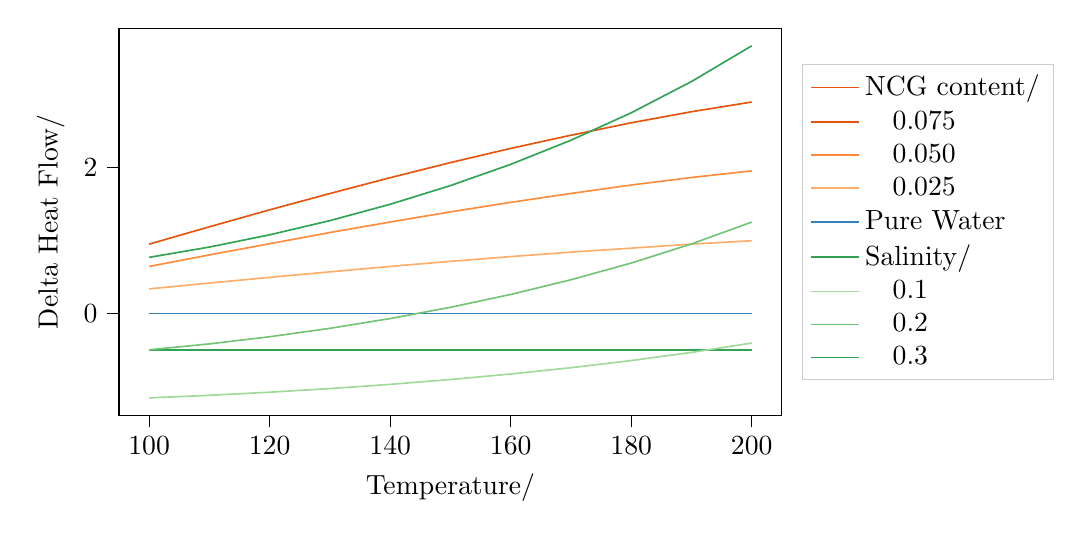
\begin{tikzpicture}

\definecolor{coral25314160}{RGB}{253,141,60}
\definecolor{darkgray176}{RGB}{176,176,176}
\definecolor{darkseagreen116196118}{RGB}{116,196,118}
\definecolor{lightgray204}{RGB}{204,204,204}
\definecolor{lightgreen161217155}{RGB}{161,217,155}
\definecolor{orangered2308513}{RGB}{230,85,13}
\definecolor{sandybrown253174107}{RGB}{253,174,107}
\definecolor{seagreen4916384}{RGB}{49,163,84}
\definecolor{steelblue49130189}{RGB}{49,130,189}

\begin{axis}[
legend cell align={left},
legend style={
  fill opacity=0.8,
  draw opacity=1,
  text opacity=1,
  at={(1.03,0.5)},
  anchor=west,
  draw=lightgray204
},
tick align=outside,
tick pos=left,
x grid style={darkgray176},
xlabel={Temperature/\unit{\degreeCelsius}},
xmin=95, xmax=205,
xtick style={color=black},
y grid style={darkgray176},
ylabel={Delta Heat Flow/\unit{\percent}},
ymin=-1.39725884403236, ymax=3.90094438467001,
ytick style={color=black},
width=10cm, height=6.5cm
]
\addplot [semithick, orangered2308513]
table {%
100 -0.5
110 -0.5
120 -0.5
130 -0.5
140 -0.5
150 -0.5
160 -0.5
170 -0.5
180 -0.5
190 -0.5
200 -0.5
};
\addlegendentry{NCG content/\unit{\kg\per\kg}}
\addplot [semithick, orangered2308513]
table {%
100 0.946972911413679
110 1.18424392033392
120 1.41644552150046
130 1.63932683056198
140 1.85603202720328
150 2.06261090261397
160 2.25676298270778
170 2.43702981631009
180 2.60717831888078
190 2.75868296786039
200 2.89124087095927
};
\addlegendentry{\quad0.075}
\addplot [semithick, coral25314160]
table {%
100 0.641500053668009
110 0.800148585333682
120 0.95280232810584
130 1.10601042046981
140 1.24987755924573
150 1.38843086822893
160 1.51879132729662
170 1.64026538799675
180 1.75564487267748
190 1.85875202501793
200 1.94965593792722
};
\addlegendentry{\quad0.050}
\addplot [semithick, sandybrown253174107]
table {%
100 0.334917798829082
110 0.414624722820633
120 0.492419823541601
130 0.567927608013052
140 0.642084636075668
150 0.711786888647059
160 0.776429515430443
170 0.837170004033716
180 0.892299335556879
190 0.947566168466629
200 0.994084695774733
};
\addlegendentry{\quad0.025}
\addplot [semithick, steelblue49130189]
table {%
100 0
110 0
120 0
130 0
140 0
150 0
160 0
170 0
180 0
190 0
200 0
};
\addlegendentry{Pure Water}
\addplot [semithick, seagreen4916384]
table {%
100 -0.5
110 -0.5
120 -0.5
130 -0.5
140 -0.5
150 -0.5
160 -0.5
170 -0.5
180 -0.5
190 -0.5
200 -0.5
};
\addlegendentry{Salinity/\unit{\kg\per\kg}}
\addplot [semithick, lightgreen161217155]
table {%
100 -1.15643142454589
110 -1.12101293316309
120 -1.0785727800762
130 -1.02877803059441
140 -0.97114586941317
150 -0.905013510669539
160 -0.829507669997931
170 -0.743499179094675
180 -0.645549510780064
190 -0.53383677112917
200 -0.406060889160786
};
\addlegendentry{\quad0.1}
\addplot [semithick, darkseagreen116196118]
table {%
100 -0.498530369472294
110 -0.417538739330847
120 -0.319831353124334
130 -0.204661458596656
140 -0.0709244192296676
150 0.0829081186268121
160 0.258867089470671
170 0.459585993949019
180 0.688431060417716
190 0.949673458609124
200 1.24871542456848
};
\addlegendentry{\quad0.2}
\addplot [semithick, seagreen4916384]
table {%
100 0.766029237295895
110 0.907206137326422
120 1.07432666748657
130 1.26874711224931
140 1.49238538931435
150 1.74783270195655
160 2.0384854742781
170 2.3687124247
180 2.74406970507353
190 3.17158207423769
200 3.66011696518354
};
\addlegendentry{\quad0.3}
\end{axis}

\end{tikzpicture}

        \caption[Deviation of liquid and vapour heat flow from pure water/steam for a range of effective salinity and \ac{NCG} content.]{Deviation of liquid and vapour heat flow from pure water/steam for a range of effective salinity and \ac{NCG} content, at a steam quality of \qty{10}{\percent}, as a function of temperature. The reference conditions are \qty{25}{\degreeCelsius} and \qty{1}{\bar}.}
        \label{fig:prosim_aspen_Heatflow}
    \end{figure}

\subsection{ELECNRTL vs. SP2009}
    Within \emph{Aspen Plus v11}, the ELECNRTL model has so far been used to capture the phase behaviour of water, sodium chloride and carbon dioxide mixtures. Given the particular focus of this work on the thermophysical properties and phase behaviour of the geofluid, it was important to compare the ELECNRTL model against other available models, such as \ac{SP2009}.

    To compare the mutual solubilities of water and carbon dioxide from the ELECNRTL model, a simple process was modelled in \emph{Aspen Plus v11}. Two streams of pure water and carbon dioxide are mixed, then taken to the desired temperature and pressure in the Heater element. Finally the mixture is partitioned into a vapour and liquid phase in the Separator, see Figure~\ref{fig:SP2009vsAspen_process_diagram}. 

    The methodology above relies on a two-phase mixture to exist at the desired temperature and pressure, such that both the liquid and vapour phase are considered saturated. For conditions, where only a single phase exists, water or carbon dioxide, would need to be added until mixture becomes saturated, however, this procedure is difficult to implement in \emph{Aspen Plus v11}. In this respect, the ratio of water to carbon dioxide at the inlet was set to 1 to 10 on a mole basis as this was found to yield a two-phase mixture over a wide range of conditions.

    \begin{figure}[H]
        \centering
        \includegraphics{Content/TPPM/CaseStudies/Figures/Aspen11vsSP2009_process_diagram.png}
        \caption{Process flow diagram of the \emph{Aspen Plus v11} simulation used to calculate the mutual solubilities of water and carbon dioxide}
        \label{fig:SP2009vsAspen_process_diagram}
    \end{figure}

    Comparing the equilibrium mole fraction of water in the vapour/carbon dioxide-rich phase, see Figures~\ref{fig:SP2009vsAspen_yH2O}, it can be seen that the ELECNRTL model generally provides higher estimates than the \ac{SP2009} model. The deviations from \ac{SP2009}'s estimates increase with decreasing temperature; from a ratio of \num{1.31} at \qty{250}{\degreeCelsius} and \qty{600}{\bar} to \num{2.20} at \qty{60}{\degreeCelsius} and \qty{600}{\bar}.
    
    \begin{figure}[H]
        \centering
        % This file was created with tikzplotlib v0.10.1.
\begin{tikzpicture}

\definecolor{crimson2143940}{RGB}{214,39,40}
\definecolor{darkgray176}{RGB}{176,176,176}
\definecolor{darkorange25512714}{RGB}{255,127,14}
\definecolor{forestgreen4416044}{RGB}{44,160,44}
\definecolor{lightgray204}{RGB}{204,204,204}
\definecolor{mediumpurple148103189}{RGB}{148,103,189}
\definecolor{orchid227119194}{RGB}{227,119,194}
\definecolor{sienna1408675}{RGB}{140,86,75}
\definecolor{steelblue31119180}{RGB}{31,119,180}

\begin{axis}[
legend cell align={left},
legend style={
  fill opacity=0.8,
  draw opacity=1,
  text opacity=1,
  at={(1.03,0.5)},
  anchor=west,
  draw=lightgray204
},
log basis x={10},
log basis y={10},
tick align=outside,
tick pos=left,
unbounded coords=jump,
x grid style={darkgray176},
xlabel={Pressure/\unit{\bar}},
xmin=1, xmax=1000,
xmode=log,
xtick style={color=black},
xtick={0.01,0.1,1,10,100,1000,10000},
xticklabels={
  \(\displaystyle {10^{-2}}\),
  \(\displaystyle {10^{-1}}\),
  \(\displaystyle {10^{0}}\),
  \(\displaystyle {10^{1}}\),
  \(\displaystyle {10^{2}}\),
  \(\displaystyle {10^{3}}\),
  \(\displaystyle {10^{4}}\)
},
y grid style={darkgray176},
ylabel={\(y_{H_2O}\)/\unit{\percent}},
ymin=0.0126543843365414, ymax=6115.23386006851,
ymode=log,
ytick style={color=black},
ytick={0.001,0.01,0.1,1,10,100,1000,10000,100000},
yticklabels={
  \(\displaystyle {10^{-3}}\),
  \(\displaystyle {10^{-2}}\),
  \(\displaystyle {10^{-1}}\),
  \(\displaystyle {10^{0}}\),
  \(\displaystyle {10^{1}}\),
  \(\displaystyle {10^{2}}\),
  \(\displaystyle {10^{3}}\),
  \(\displaystyle {10^{4}}\),
  \(\displaystyle {10^{5}}\)
},
width=10cm, height=6.5cm
]
\addplot [semithick, black, dashed]
table {%
0.1 1000
0.1 1000
};
\addlegendentry{Aspen Plus v11}
\addplot [semithick, black]
table {%
0.1 1000
0.1 1000
};
\addlegendentry{SP2009}
\addplot [semithick, steelblue31119180]
table {%
1 3373.19628441501
1.13945443811362 2960.57440652025
1.29835641653683 2596.61026399792
1.47941798107619 2273.88479876632
1.68572938436235 1984.66315199842
1.92081182847022 1718.36015421073
2.18867756273154 1460.52998183261
2.49389836245415 1207.44227609138
2.84168355730268 996.020629281356
3.23796894108304 854.848556247554
3.68951808039113 761.034876295503
4.20403775120212 687.309824728934
4.79030947360446 621.8730754414
5.45833938963633 561.399093104249
6.2195290422515 505.16871623835
7.08686997017003 453.053927303501
8.07516543984439 405.034011430344
9.20128309893242 361.091688473493
10.4844428634184 321.176883683117
11.9465449518708 285.183958633531
13.612543665533 252.941373060122
15.5108732937071 224.216503676891
17.6739334135326 198.732710581511
20.1386418669743 176.191533024508
22.9470648529046 156.29308290988
26.1471348883233 138.750803287338
29.7934688924555 123.299998795865
33.9483003563085 109.701406675184
38.6825415074099 97.7415617855309
44.0769935981326 87.2314373359878
50.2237259740978 78.0043571115077
57.2276474597881 69.9137494615865
65.2082968808572 62.8310245446456
74.3018832827234 56.6436892912557
84.6636106666994 51.2537299917828
96.4703269208944 46.5762548077101
109.923542156285 42.5383723592239
125.252867963149 39.0782698446046
142.719936287069 36.1444290850645
162.622864809594 33.6948622017724
185.301345046043 31.6961345469627
211.142440001138 30.1217489514418
240.587190333435 28.949227388388
274.138141778719 28.155174836941
312.367922305983 27.7083198587104
355.929015395883 27.5625384486293
405.56489624625 27.6541355648871
462.12272097088 27.9067937641988
526.567785363411 28.2423176640955
600 28.5909404160944
};
\addlegendentry{\qty{250}{\degreeCelsius}}
\addplot [semithick, darkorange25512714]
table {%
1 1156.51829327808
1.13945443811362 1019.55875203778
1.29835641653683 918.223639910853
1.47941798107619 830.467636835335
1.68572938436235 749.787577756501
1.92081182847022 674.750595230861
2.18867756273154 605.095654629038
2.49389836245415 540.779357945645
2.84168355730268 481.780382618666
3.23796894108304 428.044329242216
3.68951808039113 379.452343429832
4.20403775120212 335.804410506307
4.79030947360446 296.82094353616
5.45833938963633 262.160645816056
6.2195290422515 231.446827220237
7.08686997017003 204.29345954493
8.07516543984439 180.325387877163
9.20128309893242 159.191085947299
10.4844428634184 140.568971498794
11.9465449518708 124.169241146949
13.612543665533 109.733062929476
15.5108732937071 97.0304528730336
17.6739334135326 85.8576497026092
20.1386418669743 76.0344268909869
22.9470648529046 67.401549146502
26.1471348883233 59.8184530922515
29.7934688924555 53.161169305434
33.9483003563085 47.3204759549417
38.6825415074099 42.2002651367393
44.0769935981326 37.7161018702001
50.2237259740978 33.7939576977779
57.2276474597881 30.369103690498
65.2082968808572 27.3851504283947
74.3018832827234 24.7932246492538
84.6636106666994 22.5512730295482
96.4703269208944 20.6234814798429
109.923542156285 18.9797901674505
125.252867963149 17.5954637412936
142.719936287069 16.4506314929063
162.622864809594 15.5296281885145
185.301345046043 14.8198392833718
211.142440001138 14.3096470992937
240.587190333435 13.9852226437876
274.138141778719 13.8267093514817
312.367922305983 13.8057448732246
355.929015395883 13.8867278413171
405.56489624625 14.0319640869373
462.12272097088 14.2076200146599
526.567785363411 14.3872584215695
600 14.5523487339373
};
\addlegendentry{\qty{200}{\degreeCelsius}}
\addplot [semithick, forestgreen4416044]
table {%
1 450.35786229226
1.13945443811362 397.131513990463
1.29835641653683 349.906387487119
1.47941798107619 308.125780916619
1.68572938436235 271.235939429506
1.92081182847022 238.708694670326
2.18867756273154 210.054558476577
2.49389836245415 184.828409494779
2.84168355730268 162.630328380704
3.23796894108304 143.103677423025
3.68951808039113 125.931849241737
4.20403775120212 110.834537962859
4.79030947360446 97.563993058965
5.45833938963633 85.9014775370628
6.2195290422515 75.6540202415319
7.08686997017003 66.6514847331509
8.07516543984439 58.7439457492805
9.20128309893242 51.7993513201801
10.4844428634184 45.7014446348215
11.9465449518708 40.347919769229
13.612543665533 35.6487870099195
15.5108732937071 31.5249256344226
17.6739334135326 27.9068041970731
20.1386418669743 24.7333504494129
22.9470648529046 21.9509549629421
26.1471348883233 19.5125943287514
29.7934688924555 17.3770615127894
33.9483003563085 15.5082925834985
38.6825415074099 13.8747806416328
44.0769935981326 12.4490694157359
50.2237259740978 11.207320685064
57.2276474597881 10.1289514751784
65.2082968808572 9.19633877004624
74.3018832827234 8.39459095548301
84.6636106666994 7.71138526683685
96.4703269208944 7.13686618290132
109.923542156285 6.66358353874882
125.252867963149 6.28640439884998
142.719936287069 6.00222921116125
162.622864809594 5.80915563293411
185.301345046043 5.70456281150174
211.142440001138 5.68193965695884
240.587190333435 5.72788653396462
274.138141778719 5.82241939431826
312.367922305983 5.94363088834874
355.929015395883 6.07303121241615
405.56489624625 6.19781665921682
462.12272097088 6.31024286169953
526.567785363411 6.40604153370362
600 6.48306419504825
};
\addlegendentry{\qty{150}{\degreeCelsius}}
\addplot [semithick, crimson2143940]
table {%
1 95.8606316813074
1.13945443811362 84.1884141736987
1.29835641653683 73.9447949006265
1.47941798107619 64.954941917326
1.68572938436235 57.0654218702594
1.92081182847022 50.1415812997309
2.18867756273154 44.0652484707533
2.49389836245415 38.7327165096214
2.84168355730268 34.0529734252121
3.23796894108304 29.9461488082524
3.68951808039113 26.3421507006461
4.20403775120212 23.1794693736255
4.79030947360446 20.4041276034963
5.45833938963633 17.9687595358366
6.2195290422515 15.8318024260778
7.08686997017003 13.9567874741843
8.07516543984439 12.311717666945
9.20128309893242 10.8685220326594
10.4844428634184 9.60257702594147
11.9465449518708 8.49228691848849
13.612543665533 7.51871609640129
15.5108732937071 6.66526707597206
17.6739334135326 5.91739886718249
20.1386418669743 5.26238105737708
22.9470648529046 4.68907967878422
26.1471348883233 4.18777158957555
29.7934688924555 3.74998477472516
33.9483003563085 3.36836271161317
38.6825415074099 3.03655182498669
44.0769935981326 2.74911220144044
50.2237259740978 2.50145334404371
57.2276474597881 2.28979912833264
65.2082968808572 2.11118967341309
74.3018832827234 1.96353279528713
84.6636106666994 1.84572267611708
96.4703269208944 1.75783917595871
109.923542156285 1.70138755229428
125.252867963149 1.67929514914175
142.719936287069 1.69465815522904
162.622864809594 1.74651313149671
185.301345046043 1.82453677280605
211.142440001138 1.91194331536674
240.587190333435 1.99545863397715
274.138141778719 2.06891233549542
312.367922305983 2.13057725203185
355.929015395883 2.18047725320878
405.56489624625 2.21911428797825
462.12272097088 2.24701759968249
526.567785363411 2.26462174639402
600 2.27225878878611
};
\addlegendentry{\qty{99}{\degreeCelsius}}
\addplot [semithick, mediumpurple148103189]
table {%
1 19.9873187323954
1.13945443811362 17.5572599522687
1.29835641653683 15.424634958853
1.47941798107619 13.5530454381869
1.68572938436235 11.9105483007531
1.92081182847022 10.4691105029361
2.18867756273154 9.20413060515791
2.49389836245415 8.0940189016654
2.84168355730268 7.11982895685902
3.23796894108304 6.26493426076065
3.68951808039113 5.51474448674224
4.20403775120212 4.85645651116649
4.79030947360446 4.27883594874423
5.45833938963633 3.77202547942856
6.2195290422515 3.32737670159478
7.08686997017003 2.9373026501444
8.07516543984439 2.59514847423393
9.20128309893242 2.29507808413095
10.4844428634184 2.03197485637354
11.9465449518708 1.80135473693086
13.612543665533 1.59929030964659
15.5108732937071 1.42234460898291
17.6739334135326 1.26751366099953
20.1386418669743 1.13217694751987
22.9470648529046 1.01405522604548
26.1471348883233 0.911175437586962
29.7934688924555 0.821842861823804
33.9483003563085 0.744621363395653
38.6825415074099 0.678323786272784
44.0769935981326 0.62201690294655
50.2237259740978 0.575050275710673
57.2276474597881 0.537129779041046
65.2082968808572 0.508485504797335
74.3018832827234 0.490266611237576
84.6636106666994 0.485564724278958
96.4703269208944 0.502376646537759
109.923542156285 0.559422747651799
125.252867963149 0.653396391078758
142.719936287069 0.73234236621848
162.622864809594 0.791175390862061
185.301345046043 0.837470961903073
211.142440001138 0.875459001026982
240.587190333435 0.907330047558825
274.138141778719 0.934279145060401
312.367922305983 0.956979850564411
355.929015395883 0.975809589754821
405.56489624625 0.990966892409101
462.12272097088 1.00253816153125
526.567785363411 1.01053922642512
600 1.01494358195364
};
\addlegendentry{\qty{60}{\degreeCelsius}}
\addplot [semithick, sienna1408675]
table {%
1 4.51683471711622
1.13945443811362 3.96848222173234
1.29835641653683 3.48725037329212
1.47941798107619 3.06492582733172
1.68572938436235 2.69430064650029
1.92081182847022 2.36904928338135
2.18867756273154 2.08362062459628
2.49389836245415 1.83314325404748
2.84168355730268 1.61334231890936
3.23796894108304 1.42046658018884
3.68951808039113 1.25122440375662
4.20403775120212 1.10272760069786
4.79030947360446 0.972442160301424
5.45833938963633 0.858145037361983
6.2195290422515 0.757886259832108
7.08686997017003 0.669955715171282
8.07516543984439 0.592854055821143
9.20128309893242 0.525267237895015
10.4844428634184 0.466044274326347
11.9465449518708 0.41417784664369
13.612543665533 0.368787481256889
15.5108732937071 0.329105061213603
17.6739334135326 0.29446252047195
20.1386418669743 0.264281668861185
22.9470648529046 0.238066249801743
26.1471348883233 0.215396598474587
29.7934688924555 0.19592778074906
33.9483003563085 0.179393192067036
38.6825415074099 0.165618229318464
44.0769935981326 0.154555871045265
50.2237259740978 0.146379736869834
57.2276474597881 0.141772824770119
65.2082968808572 0.143292664397778
74.3018832827234 0.317764275754135
84.6636106666994 0.343432696770958
96.4703269208944 0.362550146097316
109.923542156285 0.378571700934359
125.252867963149 0.392681512340584
142.719936287069 0.405423035840708
162.622864809594 0.417076089147238
185.301345046043 0.427787382545507
211.142440001138 0.437626535958328
240.587190333435 0.44661377725109
274.138141778719 0.454735214419107
312.367922305983 0.461952127778652
355.929015395883 0.468207233558588
405.56489624625 0.473429404703805
462.12272097088 0.477537655040954
526.567785363411 0.480444847544117
600 0.482061393794867
};
\addlegendentry{\qty{31}{\degreeCelsius}}
\addplot [semithick, orchid227119194]
table {%
1 2.35264971957208
1.13945443811362 2.06721676607966
1.29835641653683 1.81672301381666
1.47941798107619 1.59689320954923
1.68572938436235 1.40397546270596
1.92081182847022 1.23467721292662
2.18867756273154 1.08610903803006
2.49389836245415 0.955735343629354
2.84168355730268 0.841331093174557
3.23796894108304 0.740943840435379
3.68951808039113 0.65286041712844
4.20403775120212 0.575577708116548
4.79030947360446 0.507777016759015
5.45833938963633 0.44830158482439
6.2195290422515 0.396136886031587
7.08686997017003 0.350393360830532
8.07516543984439 0.310291303516491
9.20128309893242 0.275147652296223
10.4844428634184 0.244364469775067
11.9465449518708 0.217418937207
13.612543665533 0.193854723277746
15.5108732937071 0.173274631406898
17.6739334135326 0.155334486317274
20.1386418669743 0.139738306324819
22.9470648529046 0.126234955385299
26.1471348883233 0.114616754684432
29.7934688924555 0.104721151259144
33.9483003563085 0.0964380423581058
38.6825415074099 0.0897295603970565
44.0769935981326 0.0846834348272989
50.2237259740978 0.0816869744775875
57.2276474597881 0.0823716981990398
65.2082968808572 0.262472294979018
74.3018832827234 0.270557951325723
84.6636106666994 0.27818776886782
96.4703269208944 0.285469514955282
109.923542156285 0.292462141844152
125.252867963149 0.299194093038642
142.719936287069 0.305672673941479
162.622864809594 0.311889234582566
185.301345046043 0.317822225720444
211.142440001138 0.323439126999483
240.587190333435 0.328697779166832
274.138141778719 0.333547430236899
312.367922305983 0.337929692527985
355.929015395883 0.341779546157087
405.56489624625 0.345026488242659
462.12272097088 0.34759590236487
526.567785363411 0.349410702494331
600 0.350393285369793
};
\addlegendentry{\qty{20}{\degreeCelsius}}
\addplot [semithick, steelblue31119180, dashed, forget plot]
table {%
1 nan
1.30543816 nan
1.70416878 nan
2.22468695 nan
2.90419122 nan
3.79124203 nan
4.949232 nan
6.4609163 nan
8.43432665 nan
11.0104918 nan
14.3735161 nan
18.7637364 nan
24.4948974 nan
31.9765737 nan
41.7434394 nan
54.4934785 76.7984284
71.1378661 62.3061543
92.8660847 51.4784731
121.23093 43.63366
158.259482 38.3348659
206.597966 35.3797986
269.700868 34.68412
352.077804 35.6423097
459.615798 36.8649336
600 37.4712302
};
\addplot [semithick, darkorange25512714, dashed, forget plot]
table {%
1 nan
1.30543816 nan
1.70416878 nan
2.22468695 nan
2.90419122 nan
3.79124203 nan
4.949232 nan
6.4609163 nan
8.43432665 nan
11.0104918 nan
14.3735161 nan
18.7637364 83.9000243
24.4948974 65.8213751
31.9765737 51.9947908
41.7434394 41.4614556
54.4934785 33.48904
71.1378661 27.524002
92.8660847 23.1713889
121.23093 20.1725313
158.259482 18.3888823
206.597966 17.7916596
269.700868 18.2592387
352.077804 19.2682148
459.615798 20.1780966
600 20.6859035
};
\addplot [semithick, forestgreen4416044, dashed, forget plot]
table {%
1 nan
1.30543816 nan
1.70416878 nan
2.22468695 nan
2.90419122 nan
3.79124203 nan
4.949232 nan
6.4609163 74.2482788
8.43432665 57.4692029
11.0104918 44.6134907
14.3735161 34.7727646
18.7637364 27.2455532
24.4948974 21.5018428
31.9765737 17.1348321
41.7434394 13.8261116
54.4934785 11.3589038
71.1378661 9.5627172
92.8660847 8.33124835
121.23093 7.62602411
158.259482 7.47430133
206.597966 7.90621816
269.700868 8.72002513
352.077804 9.51917344
459.615798 10.1091906
600 10.451141
};
\addplot [semithick, crimson2143940, dashed, forget plot]
table {%
1 nan
1.30543816 75.0774333
1.70416878 57.6743116
2.22468695 44.3396329
2.90419122 34.1244948
3.79124203 26.2996104
4.949232 20.3054286
6.4609163 15.71746
8.43432665 12.2044791
11.0104918 9.51744011
14.3735161 7.46373554
18.7637364 5.89802023
24.4948974 4.70864877
31.9765737 3.81234196
41.7434394 3.1459413
54.4934785 2.66848699
71.1378661 2.3562028
92.8660847 2.2140027
121.23093 2.29697691
158.259482 2.70948901
206.597966 3.30966709
269.700868 3.82468614
352.077804 4.2137009
459.615798 4.488278
600 4.6553549
};
\addplot [semithick, mediumpurple148103189, dashed, forget plot]
table {%
1 20.1218616
1.30543816 15.4556028
1.70416878 11.8814474
2.22468695 9.1436424
2.90419122 7.04657104
3.79124203 5.44062675
4.949232 4.21092417
6.4609163 3.26976322
8.43432665 2.54994356
11.0104918 2.00002175
14.3735161 1.58078533
18.7637364 1.26252113
24.4948974 1.02290536
31.9765737 0.845604916
41.7434394 0.719814474
54.4934785 0.640780576
71.1378661 0.616115247
92.8660847 0.697989773
121.23093 1.0852623
158.259482 1.45801127
206.597966 1.71473199
269.700868 1.91194013
352.077804 2.06630463
459.615798 2.18004756
600 2.25097997
};
\addplot [semithick, sienna1408675, dashed, forget plot]
table {%
1 4.56234095
1.30543816 3.5065469
1.70416878 2.69781338
2.22468695 2.07839741
2.90419122 1.60403408
3.79124203 1.24082531
4.949232 0.962817969
6.4609163 0.750163637
8.43432665 0.587702044
11.0104918 0.463803306
14.3735161 0.369695335
18.7637364 0.298775015
24.4948974 0.246215205
31.9765737 0.208880925
41.7434394 0.185294769
54.4934785 0.178621908
71.1378661 0.229108887
92.8660847 0.195699226
121.23093 0.157508577
158.259482 0.125762562
206.597966 0.100387976
269.700868 0.0805893448
352.077804 0.0654485219
459.615798 0.0540875656
600 0.0458457638
};
\addplot [semithick, orchid227119194, dashed, forget plot]
table {%
1 2.37790553
1.30543816 1.82811645
1.70416878 1.40700803
2.22468695 1.08448625
2.90419122 0.837502255
3.79124203 0.648405269
4.949232 0.503694336
6.4609163 0.393105375
8.43432665 0.308610612
11.0104918 0.244251419
14.3735161 0.195480671
18.7637364 0.158875684
24.4948974 0.132050477
31.9765737 0.113612919
41.7434394 0.103343085
54.4934785 0.106454451
71.1378661 0.119686933
92.8660847 0.0983175743
121.23093 0.0789271052
158.259482 0.0628608871
206.597966 0.0501321653
269.700868 0.0402180678
352.077804 0.0326626227
459.615798 0.0270086968
600 0.022941007
};
\end{axis}

\end{tikzpicture}
         
        \caption[Comparison of the equilibrium mole fraction of water in a carbon dioxide-rich phase predictions.]{The equilibrium mole fraction of water in a carbon dioxide-rich phase as a function of temperature and pressure, as calculated using the ELECNRTL model in \emph{Aspen Plus v11} and the \ac{SP2009} model}
        \label{fig:SP2009vsAspen_yH2O}
    \end{figure}

    The observed deviations at temperatures below \qty{60}{\degreeCelsius} can in part be explained by phase change of the carbon dioxide-rich phase from vapour to liquid, visible as the discontinuities of the lines corresponding to temperatures of \qty{31}{\degreeCelsius} and \qty{20}{\degreeCelsius}. This phase change does not appear to be captured within the ELECNRTL model in \emph{Aspen Plus v11}. 
    
    % \begin{figure}[H]
    %     \centering
    %     \input{Content/ProSim/AspenPlus/Plots/ELECNRTLvsSP2009/SP2009vsAspen_yH2O_log_ratio}         
    %     \caption{The ratio of equilibrium mole fractions of water in a carbon dioxide-rich phase, as a function of temperature and pressure, as calculated using the ELECNRTL model in \emph{Aspen Plus v11} and the \ac{SP2009} model}
    %     \label{fig:SP2009vsAspen_yH2O_ratio}
    % \end{figure}

    As for the equilibrium mole fraction of carbon dioxide in a water-rich phase, while the ELECNRTL and \ac{SP2009} models show good agreement at low temperatures, they deviate considerably at higher temperatures, see Figures~\ref{fig:SP2009vsAspen_xCO2_part2} and \ref{fig:SP2009vsAspen_xCO2_part1}. As described above, the low-temperature and high-pressure behaviour of the ELECNRTL model can likely be attributed to the phase change from vapour to liquid carbon dioxide not being captured.
    
    \begin{figure}[H]
        \centering
        % This file was created with tikzplotlib v0.10.1.
\begin{tikzpicture}

\definecolor{crimson2143940}{RGB}{214,39,40}
\definecolor{darkgray176}{RGB}{176,176,176}
\definecolor{darkorange25512714}{RGB}{255,127,14}
\definecolor{forestgreen4416044}{RGB}{44,160,44}
\definecolor{lightgray204}{RGB}{204,204,204}
\definecolor{steelblue31119180}{RGB}{31,119,180}

\begin{axis}[
legend cell align={left},
legend style={
  fill opacity=0.8,
  draw opacity=1,
  text opacity=1,
  at={(1.03,0.5)},
  anchor=west,
  draw=lightgray204
},
log basis x={10},
tick align=outside,
tick pos=left,
unbounded coords=jump,
x grid style={darkgray176},
xlabel={Pressure/\unit{\bar}},
xmin=1, xmax=1000,
xmode=log,
xtick style={color=black},
xtick={0.01,0.1,1,10,100,1000,10000},
xticklabels={
  \(\displaystyle {10^{-2}}\),
  \(\displaystyle {10^{-1}}\),
  \(\displaystyle {10^{0}}\),
  \(\displaystyle {10^{1}}\),
  \(\displaystyle {10^{2}}\),
  \(\displaystyle {10^{3}}\),
  \(\displaystyle {10^{4}}\)
},
y grid style={darkgray176},
ylabel={\(x_{CO_2}\)/\unit{\percent}},
ymin=0, ymax=10,
ytick style={color=black},
width=10cm, height=6cm
]
\addplot [semithick, black, dashed]
table {%
0.1 1000
0.1 1000
};
\addlegendentry{Aspen Plus v11}
\addplot [semithick, black]
table {%
0.1 1000
0.1 1000
};
\addlegendentry{SP2009}
\addplot [semithick, steelblue31119180]
table {%
1 -0.653841086378044
1.13945443811362 -0.639977912981851
1.29835641653683 -0.629536756553862
1.47941798107619 -0.61920677137267
1.68572938436235 -0.607199532350994
1.92081182847022 -0.592524966880268
2.18867756273154 -0.574441048478481
2.49389836245415 -0.553488382736491
2.84168355730268 -0.533858444920141
3.23796894108304 -0.519814865831549
3.68951808039113 -0.510590837438871
4.20403775120212 -0.503336774867244
4.79030947360446 -0.496221871570127
5.45833938963633 -0.488436070804888
6.2195290422515 -0.47957595266589
7.08686997017003 -0.469318009911993
8.07516543984439 -0.457309495908206
9.20128309893242 -0.443143725975259
10.4844428634184 -0.426361648768918
11.9465449518708 -0.406460837871598
13.612543665533 -0.382904053106502
15.5108732937071 -0.355122419881978
17.6739334135326 -0.322511093296748
20.1386418669743 -0.284418265703673
22.9470648529046 -0.240129998325265
26.1471348883233 -0.188853266951984
29.7934688924555 -0.129698652956862
33.9483003563085 -0.0616631835323898
38.6825415074099 0.016386692244764
44.0769935981326 0.105732136287345
50.2237259740978 0.207818997289116
57.2276474597881 0.324274718714433
65.2082968808572 0.456924532950762
74.3018832827234 0.607805969248388
84.6636106666994 0.779180171209233
96.4703269208944 0.973537885910133
109.923542156285 1.19359732258776
125.252867963149 1.44229061812427
142.719936287069 1.72273597144024
162.622864809594 2.03819488439619
185.301345046043 2.39202083047252
211.142440001138 2.7876211853091
240.587190333435 3.22848356232278
274.138141778719 3.71836237836517
312.367922305983 4.26176671751886
355.929015395883 4.86488973296516
405.56489624625 5.53701486549281
462.12272097088 6.29225186143922
526.567785363411 7.15135760056152
600 8.14344582145374
};
\addlegendentry{\qty{250}{\degreeCelsius}}
\addplot [semithick, darkorange25512714]
table {%
1 -0.209830680589779
1.13945443811362 -0.206672465150957
1.29835641653683 -0.204343195219421
1.47941798107619 -0.202148885090668
1.68572938436235 -0.199781094358791
1.92081182847022 -0.197100753861871
2.18867756273154 -0.194007946830008
2.49389836245415 -0.190397637726997
2.84168355730268 -0.186149087537316
3.23796894108304 -0.181125453777519
3.68951808039113 -0.175176251384995
4.20403775120212 -0.168140037777978
4.79030947360446 -0.15984576527303
5.45833938963633 -0.15011201325226
6.2195290422515 -0.138744184759723
7.08686997017003 -0.125530315986764
8.07516543984439 -0.110236220209321
9.20128309893242 -0.0926004543785929
10.4844428634184 -0.0723293195778993
11.9465449518708 -0.0490919246886503
13.612543665533 -0.0225152699266934
15.5108732937071 0.00782069267966676
17.6739334135326 0.0423880263115314
20.1386418669743 0.081715750718756
22.9470648529046 0.126394633524274
26.1471348883233 0.177081620021581
29.7934688924555 0.234503581237518
33.9483003563085 0.299459922013575
38.6825415074099 0.372823415557409
44.0769935981326 0.455538411046307
50.2237259740978 0.548615292337232
57.2276474597881 0.653119752715694
65.2082968808572 0.770155114669575
74.3018832827234 0.900835621964688
84.6636106666994 1.04624848705273
96.4703269208944 1.20740273071647
109.923542156285 1.38516393869656
125.252867963149 1.58017671018863
142.719936287069 1.79278186466946
162.622864809594 2.02294464393256
185.301345046043 2.2702235830944
211.142440001138 2.53382409733677
240.587190333435 2.81278394393854
274.138141778719 3.10630646466055
312.367922305983 3.41417681982969
355.929015395883 3.73710698542361
405.56489624625 4.07685783592469
462.12272097088 4.43611451500369
526.567785363411 4.81822065280279
600 5.22688825336974
};
\addlegendentry{\qty{200}{\degreeCelsius}}
\addplot [semithick, forestgreen4416044]
table {%
1 -0.0609944522738537
1.13945443811362 -0.0588783927944637
1.29835641653683 -0.0564045253951016
1.47941798107619 -0.0535250725040262
1.68572938436235 -0.0501872360360478
1.92081182847022 -0.0463319701527379
2.18867756273154 -0.0418927083608173
2.49389836245415 -0.0367940569943088
2.84168355730268 -0.0309504390221846
3.23796894108304 -0.0242646617015433
3.68951808039113 -0.0166263811129694
4.20403775120212 -0.00791044041366548
4.79030947360446 0.00202493605584547
5.45833938963633 0.0133401047069528
6.2195290422515 0.0262161257633246
7.08686997017003 0.0408570442361912
8.07516543984439 0.057492314956856
9.20128309893242 0.0763793437503298
10.4844428634184 0.0978060980969823
11.9465449518708 0.122093715678384
13.612543665533 0.149599006172738
15.5108732937071 0.180716698299916
17.6739334135326 0.215881227738877
20.1386418669743 0.25556778906762
22.9470648529046 0.300292282933201
26.1471348883233 0.350609674883038
29.7934688924555 0.407110141962441
33.9483003563085 0.470412216465029
38.6825415074099 0.541151946394881
44.0769935981326 0.619966890677415
50.2237259740978 0.707473580502984
57.2276474597881 0.804236960250663
65.2082968808572 0.910730374173663
74.3018832827234 1.0272850738227
84.6636106666994 1.15402931336516
96.4703269208944 1.29081943556018
109.923542156285 1.43716983839833
125.252867963149 1.59219664938918
142.719936287069 1.75460253174629
162.622864809594 1.92274599987058
185.301345046043 2.09484689221178
211.142440001138 2.26934876630732
240.587190333435 2.44535198232017
274.138141778719 2.6228990096453
312.367922305983 2.80292784922501
355.929015395883 2.98695897799016
405.56489624625 3.17674725110351
462.12272097088 3.37404582125602
526.567785363411 3.58048485599962
600 3.79751201982416
};
\addlegendentry{\qty{150}{\degreeCelsius}}
\addplot [semithick, crimson2143940]
table {%
1 0.000842091372508321
1.13945443811362 0.00366345772156311
1.29835641653683 0.00687498985999162
1.47941798107619 0.0105301205808869
1.68572938436235 0.0146894438550586
1.92081182847022 0.0194216275560075
2.18867756273154 0.0248044281491446
2.49389836245415 0.030925814162754
2.84168355730268 0.0378852040730069
3.23796894108304 0.0457948222819718
3.68951808039113 0.0547811738752559
4.20403775120212 0.064986634464907
4.79030947360446 0.0765711452050088
5.45833938963633 0.089713994441227
6.2195290422515 0.10461565570101
7.08686997017003 0.121499635947259
8.07516543984439 0.140614267090361
9.20128309893242 0.162234346319772
10.4844428634184 0.186662495239121
11.9465449518708 0.214230062137678
13.612543665533 0.245297333790684
15.5108732937071 0.28025275050416
17.6739334135326 0.319510728157049
20.1386418669743 0.363507581350716
22.9470648529046 0.412694910677971
26.1471348883233 0.467529664212294
29.7934688924555 0.528459910993262
33.9483003563085 0.595905179960589
38.6825415074099 0.670230037760589
44.0769935981326 0.751709435179402
50.2237259740978 0.840484305543162
57.2276474597881 0.936506065701868
65.2082968808572 1.03946928239895
74.3018832827234 1.14873331147446
84.6636106666994 1.26323729583121
96.4703269208944 1.38142115527017
109.923542156285 1.50118449029363
125.252867963149 1.61995921359021
142.719936287069 1.73505218217708
162.622864809594 1.84444243040359
185.301345046043 1.94779328655861
211.142440001138 2.0466217408854
240.587190333435 2.14327252271507
274.138141778719 2.23993502877001
312.367922305983 2.33834838698105
355.929015395883 2.43986090841645
405.56489624625 2.54554373136545
462.12272097088 2.65627373672423
526.567785363411 2.77278047392794
600 2.89566559681683
};
\addlegendentry{\qty{99}{\degreeCelsius}}
\addplot [semithick, steelblue31119180, dashed, forget plot]
table {%
1 nan
1.30543816 nan
1.70416878 nan
2.22468695 nan
2.90419122 nan
3.79124203 nan
4.949232 nan
6.4609163 nan
8.43432665 nan
11.0104918 nan
14.3735161 nan
18.7637364 nan
24.4948974 nan
31.9765737 nan
41.7434394 nan
54.4934785 0.213602393
71.1378661 0.448842376
92.8660847 0.745290452
121.23093 1.10965743
158.259482 1.53991563
206.597966 2.0063757
269.700868 2.43524648
352.077804 2.7095663
459.615798 2.73751778
600 2.50691772
};
\addplot [semithick, darkorange25512714, dashed, forget plot]
table {%
1 nan
1.30543816 nan
1.70416878 nan
2.22468695 nan
2.90419122 nan
3.79124203 nan
4.949232 nan
6.4609163 nan
8.43432665 nan
11.0104918 nan
14.3735161 nan
18.7637364 0.0447417211
24.4948974 0.122706488
31.9765737 0.222245297
41.7434394 0.348161283
54.4934785 0.50552179
71.1378661 0.698684619
92.8660847 0.929256961
121.23093 1.19228276
158.259482 1.47120876
206.597966 1.73330509
269.700868 1.9338488
352.077804 2.03575831
459.615798 2.02129437
600 1.88524523
};
\addplot [semithick, forestgreen4416044, dashed, forget plot]
table {%
1 nan
1.30543816 nan
1.70416878 nan
2.22468695 nan
2.90419122 nan
3.79124203 nan
4.949232 nan
6.4609163 0.0243098532
8.43432665 0.0521000416
11.0104918 0.0880011224
14.3735161 0.1341864
18.7637364 0.193361602
24.4948974 0.268699338
31.9765737 0.363696699
41.7434394 0.482417002
54.4934785 0.627742314
71.1378661 0.801559517
92.8660847 1.00198535
121.23093 1.21983707
158.259482 1.43789752
206.597966 1.63024709
269.700868 1.77918024
352.077804 1.87800835
459.615798 1.92192679
600 1.90224267
};
\addplot [semithick, crimson2143940, dashed, forget plot]
table {%
1 nan
1.30543816 0.0060493967
1.70416878 0.013347286
2.22468695 0.0228321992
2.90419122 0.0351636858
3.79124203 0.0511549794
4.949232 0.071883732
6.4609163 0.0987231506
8.43432665 0.133278569
11.0104918 0.177671153
14.3735161 0.23454185
18.7637364 0.306668642
24.4948974 0.39740976
31.9765737 0.510085645
41.7434394 0.64762426
54.4934785 0.810901049
71.1378661 0.997540267
92.8660847 1.19879819
121.23093 1.39544009
158.259482 1.56318506
206.597966 1.69347999
269.700868 1.79830562
352.077804 1.88408078
459.615798 1.95028623
600 1.98935022
};
\end{axis}

\end{tikzpicture}

        \caption[Comparison of the equilibrium mole fraction of carbon dioxide in a water-rich phase predictions. Part 1.]{The equilibrium mole fraction of carbon dioxide in a water-rich phase as a function of temperature and pressure, as calculated using the ELECNRTL model in \emph{Aspen Plus v11} and the \ac{SP2009} model}
        \label{fig:SP2009vsAspen_xCO2_part2}
    \end{figure}
    \begin{figure}[H]
        \centering
        % This file was created with tikzplotlib v0.10.1.
\begin{tikzpicture}

\definecolor{crimson2143940}{RGB}{214,39,40}
\definecolor{darkgray176}{RGB}{176,176,176}
\definecolor{lightgray204}{RGB}{204,204,204}
\definecolor{mediumpurple148103189}{RGB}{148,103,189}
\definecolor{orchid227119194}{RGB}{227,119,194}
\definecolor{sienna1408675}{RGB}{140,86,75}

\begin{axis}[
legend cell align={left},
legend style={
  fill opacity=0.8,
  draw opacity=1,
  text opacity=1,
  at={(0.03,0.97)},
  anchor=north west,
  draw=lightgray204
},
log basis x={10},
tick align=outside,
tick pos=left,
unbounded coords=jump,
x grid style={darkgray176},
xlabel={Pressure/\unit{\bar}},
xmin=0.726260522026317, xmax=826.149820626293,
xmode=log,
xtick style={color=black},
xtick={0.01,0.1,1,10,100,1000,10000},
xticklabels={
  \(\displaystyle {10^{-2}}\),
  \(\displaystyle {10^{-1}}\),
  \(\displaystyle {10^{0}}\),
  \(\displaystyle {10^{1}}\),
  \(\displaystyle {10^{2}}\),
  \(\displaystyle {10^{3}}\),
  \(\displaystyle {10^{4}}\)
},
y grid style={darkgray176},
ylabel={\(x_{CO_2}\)/\unit{\percent}},
ymin=0, ymax=10,
ytick style={color=black}
]
\addplot [semithick, black, dashed]
table {%
-1 1000
-1 1000
};
\addlegendentry{Aspen Plus v11}
\addplot [semithick, black]
table {%
-1 1000
-1 1000
};
\addlegendentry{SP2009}
\addplot [semithick, crimson2143940]
table {%
1 0.000842091372508321
1.13945443811362 0.00366345772156311
1.29835641653683 0.00687498985999162
1.47941798107619 0.0105301205808869
1.68572938436235 0.0146894438550586
1.92081182847022 0.0194216275560075
2.18867756273154 0.0248044281491446
2.49389836245415 0.030925814162754
2.84168355730268 0.0378852040730069
3.23796894108304 0.0457948222819718
3.68951808039113 0.0547811738752559
4.20403775120212 0.064986634464907
4.79030947360446 0.0765711452050088
5.45833938963633 0.089713994441227
6.2195290422515 0.10461565570101
7.08686997017003 0.121499635947259
8.07516543984439 0.140614267090361
9.20128309893242 0.162234346319772
10.4844428634184 0.186662495239121
11.9465449518708 0.214230062137678
13.612543665533 0.245297333790684
15.5108732937071 0.28025275050416
17.6739334135326 0.319510728157049
20.1386418669743 0.363507581350716
22.9470648529046 0.412694910677971
26.1471348883233 0.467529664212294
29.7934688924555 0.528459910993262
33.9483003563085 0.595905179960589
38.6825415074099 0.670230037760589
44.0769935981326 0.751709435179402
50.2237259740978 0.840484305543162
57.2276474597881 0.936506065701868
65.2082968808572 1.03946928239895
74.3018832827234 1.14873331147446
84.6636106666994 1.26323729583121
96.4703269208944 1.38142115527017
109.923542156285 1.50118449029363
125.252867963149 1.61995921359021
142.719936287069 1.73505218217708
162.622864809594 1.84444243040359
185.301345046043 1.94779328655861
211.142440001138 2.0466217408854
240.587190333435 2.14327252271507
274.138141778719 2.23993502877001
312.367922305983 2.33834838698105
355.929015395883 2.43986090841645
405.56489624625 2.54554373136545
462.12272097088 2.65627373672423
526.567785363411 2.77278047392794
600 2.89566559681683
};
\addlegendentry{\qty{99}{\degreeCelsius}}
\addplot [semithick, mediumpurple148103189]
table {%
1 0.0240980682246103
1.13945443811362 0.0282745251266536
1.29835641653683 0.033026877993203
1.47941798107619 0.0384334965086635
1.68572938436235 0.0445831032101791
1.92081182847022 0.0515760468355555
2.18867756273154 0.059525703115842
2.49389836245415 0.0685600061668129
2.84168355730268 0.0788231098717408
3.23796894108304 0.090477173182895
3.68951808039113 0.103704255546935
4.20403775120212 0.118708297969926
4.79030947360446 0.135717150677498
5.45833938963633 0.154984588752501
6.2195290422515 0.176792231113292
7.08686997017003 0.201451243947138
8.07516543984439 0.22930366503681
9.20128309893242 0.260723127632304
10.4844428634184 0.296114688391748
11.9465449518708 0.335913369603102
13.612543665533 0.38058090690156
15.5108732937071 0.430600044830597
17.6739334135326 0.486465537964968
20.1386418669743 0.548670788268976
22.9470648529046 0.617688772275085
26.1471348883233 0.693945575227912
29.7934688924555 0.777784440572882
33.9483003563085 0.869417740314168
38.6825415074099 0.968863631638488
44.0769935981326 1.07586329260649
50.2237259740978 1.18977330328974
57.2276474597881 1.30942542899887
65.2082968808572 1.43294148422634
74.3018832827234 1.55748106291853
84.6636106666994 1.67887922154745
96.4703269208944 1.79111928166653
109.923542156285 1.88619076058784
125.252867963149 1.9604893909678
142.719936287069 2.02333920491929
162.622864809594 2.0826558210044
185.301345046043 2.1416998149942
211.142440001138 2.20206825582779
240.587190333435 2.26474531696006
274.138141778719 2.33044100767523
312.367922305983 2.39972155472342
355.929015395883 2.47306510254641
405.56489624625 2.55088485904988
462.12272097088 2.63353508398598
526.567785363411 2.72130601056684
600 2.81441003966434
};
\addlegendentry{\qty{60}{\degreeCelsius}}
\addplot [semithick, sienna1408675]
table {%
1 0.0492827466363969
1.13945443811362 0.0564319766004036
1.29835641653683 0.0645639486196628
1.47941798107619 0.0738114746178488
1.68572938436235 0.084324631434466
1.92081182847022 0.0962727972319106
2.18867756273154 0.109846862808871
2.49389836245415 0.125261610463398
2.84168355730268 0.142758242923519
3.23796894108304 0.162607030783053
3.68951808039113 0.185110027613429
4.20403775120212 0.210603775895751
4.79030947360446 0.239461892134059
5.45833938963633 0.272097373446832
6.2195290422515 0.308964407417498
7.08686997017003 0.350559388047301
8.07516543984439 0.397420738349136
9.20128309893242 0.450127008294896
10.4844428634184 0.50929254780944
11.9465449518708 0.575559838640007
13.612543665533 0.649587293823883
15.5108732937071 0.732030982572552
17.6739334135326 0.82351828813462
20.1386418669743 0.924610920011274
22.9470648529046 1.03575391673211
26.1471348883233 1.15720617049384
29.7934688924555 1.28894632537434
33.9483003563085 1.43054505772893
38.6825415074099 1.58098924865883
44.0769935981326 1.73843117748235
50.2237259740978 1.89980265954622
57.2276474597881 2.0601220050466
65.2082968808572 2.2107635569298
74.3018832827234 2.29375983077898
84.6636106666994 2.32510066217716
96.4703269208944 2.35732938791603
109.923542156285 2.3911688354176
125.252867963149 2.42707602007208
142.719936287069 2.46541369000824
162.622864809594 2.50650405127708
185.301345046043 2.55065019829834
211.142440001138 2.59814514391716
240.587190333435 2.6492747409016
274.138141778719 2.70431677245408
312.367922305983 2.76353700007062
355.929015395883 2.82718228766096
405.56489624625 2.89547055636822
462.12272097088 2.96857708513498
526.567785363411 3.04661649063404
600 3.12961957499624
};
\addlegendentry{\qty{31}{\degreeCelsius}}
\addplot [semithick, orchid227119194]
table {%
1 0.0653247926336365
1.13945443811362 0.0745852094002488
1.29835641653683 0.0851166689054567
1.47941798107619 0.097090371394312
1.68572938436235 0.110699597084132
1.92081182847022 0.126162255128633
2.18867756273154 0.143723632350198
2.49389836245415 0.163659324314376
2.84168355730268 0.18627831592281
3.23796894108304 0.21192615753484
3.68951808039113 0.240988153919776
4.20403775120212 0.273892444826732
4.79030947360446 0.311112804759125
5.45833938963633 0.353170922013027
6.2195290422515 0.400637828584968
7.08686997017003 0.454134037383873
8.07516543984439 0.514327793993338
9.20128309893242 0.581930657775951
10.4844428634184 0.657689379529053
11.9465449518708 0.742372724610481
13.612543665533 0.836751480141146
15.5108732937071 0.941569351562593
17.6739334135326 1.05750174854906
20.1386418669743 1.18509849803247
22.9470648529046 1.32470513983392
26.1471348883233 1.47635531414414
29.7934688924555 1.63962304397092
33.9483003563085 1.81341641616122
38.6825415074099 1.99567740705381
44.0769935981326 2.18290640121608
50.2237259740978 2.36926618803906
57.2276474597881 2.54410251378048
65.2082968808572 2.52015780659073
74.3018832827234 2.54303978477881
84.6636106666994 2.5678533946345
96.4703269208944 2.59480927837136
109.923542156285 2.62412239648652
125.252867963149 2.65601445284037
142.719936287069 2.69071480655795
162.622864809594 2.72846028353984
185.301345046043 2.7694939890957
211.142440001138 2.81406305754705
240.587190333435 2.86241516307756
274.138141778719 2.91479352271017
312.367922305983 2.97143003141135
355.929015395883 3.03253607395257
405.56489624625 3.09829045598115
462.12272097088 3.1688237891392
526.567785363411 3.24419855749769
600 3.32438399595852
};
\addlegendentry{\qty{20}{\degreeCelsius}}
\addplot [semithick, crimson2143940, dashed, forget plot]
table {%
1 nan
1.30543816 0.0060493967
1.70416878 0.013347286
2.22468695 0.0228321992
2.90419122 0.0351636858
3.79124203 0.0511549794
4.949232 0.071883732
6.4609163 0.0987231506
8.43432665 0.133278569
11.0104918 0.177671153
14.3735161 0.23454185
18.7637364 0.306668642
24.4948974 0.39740976
31.9765737 0.510085645
41.7434394 0.64762426
54.4934785 0.810901049
71.1378661 0.997540267
92.8660847 1.19879819
121.23093 1.39544009
158.259482 1.56318506
206.597966 1.69347999
269.700868 1.79830562
352.077804 1.88408078
459.615798 1.95028623
600 1.98935022
};
\addplot [semithick, mediumpurple148103189, dashed, forget plot]
table {%
1 0.0234478746
1.30543816 0.0323227308
1.70416878 0.0438655753
2.22468695 0.0588453738
2.90419122 0.0782878596
3.79124203 0.103465847
4.949232 0.13601389
6.4609163 0.177911395
8.43432665 0.231739678
11.0104918 0.300326713
14.3735161 0.387381199
18.7637364 0.496275111
24.4948974 0.631015627
31.9765737 0.794244727
41.7434394 0.987258201
54.4934785 1.20529824
71.1378661 1.43622926
92.8660847 1.64935318
121.23093 1.79973624
158.259482 1.90027842
206.597966 1.99100204
269.700868 2.07940795
352.077804 2.16708189
459.615798 2.25147009
600 2.32727064
};
\addplot [semithick, sienna1408675, dashed, forget plot]
table {%
1 0.0504832048
1.30543816 0.0664544837
1.70416878 0.087171495
2.22468695 0.114018717
2.90419122 0.148734811
3.79124203 0.193497996
4.949232 0.250999288
6.4609163 0.324513614
8.43432665 0.41797484
11.0104918 0.535615234
14.3735161 0.682118221
18.7637364 0.861834023
24.4948974 1.07774696
31.9765737 1.3300831
41.7434394 1.61167415
54.4934785 1.90484524
71.1378661 2.16261568
92.8660847 2.66833533
121.23093 3.27336683
158.259482 3.95971157
206.597966 4.70596578
269.700868 5.46982679
352.077804 6.18837023
459.615798 6.77106047
600 7.10473765
};
\addplot [semithick, orchid227119194, dashed, forget plot]
table {%
1 0.0695278598
1.30543816 0.0909530598
1.70416878 0.118715692
2.22468695 0.154612308
2.90419122 0.200894242
3.79124203 0.260344775
4.949232 0.336351852
6.4609163 0.432985886
8.43432665 0.554713719
11.0104918 0.70648159
14.3735161 0.89314025
18.7637364 1.11816442
24.4948974 1.38335802
31.9765737 1.68539327
41.7434394 2.01101376
54.4934785 2.32864355
71.1378661 2.73628764
92.8660847 3.35017968
121.23093 4.05218189
158.259482 4.82786712
206.597966 5.64549415
269.700868 6.46301683
352.077804 7.21384495
459.615798 7.81368413
600 8.15739397
};
\end{axis}

\end{tikzpicture}

        \caption[Comparison of the equilibrium mole fraction of carbon dioxide in a water-rich phase predictions. Part 2.]{The equilibrium mole fraction of carbon dioxide in a water-rich phase as a function of temperature and pressure, as calculated using the ELECNRTL model in \emph{Aspen Plus v11} and the \ac{SP2009} model}
        \label{fig:SP2009vsAspen_xCO2_part1}
    \end{figure}

    % \begin{figure}[H]
    %     \centering
    %     \input{Content/ProSim/AspenPlus/Plots/ELECNRTLvsSP2009/SP2009vsAspen_xCO2_log_ratio}         
    %     \caption{The ratio of equilibrium mole fractions of carbon dioxide in a water-rich phase, as a function of temperature and pressure, as calculated using the ELECNRTL model in \emph{Aspen Plus v11} and the \ac{SP2009} model}
    %     \label{fig:SP2009vsAspen_xCO2_ratio}
    % \end{figure}

    Another factor to consider when comparing these results is nature of the phases considered by each model: \emph{Aspen Plus v11} differentiates between a vapour, liquid and solid phase, whereas \ac{SP2009} considers a water-rich and a carbon dioxide-rich phase. For the vast majority of conditions these definitions are congruent, however below the critical temperature of carbon dioxide (about \qty{31}{\degreeCelsius}) carbon dioxide can exist in its liquid state, provided pressures are sufficiently high. For our investigation it is unclear, whether the ELECNRTL model makes this distinction, nevertheless, \emph{Aspen Plus v11} still reports carbon dioxide in the vapour phase at these conditions, see Figure~\ref{fig:SP2009vsAspen_supcritCO2}.

    \begin{figure}[H]
        \centering
        \frame{\includegraphics[scale=0.9]{Content/TPPM/CaseStudies/Figures/Aspen11vsSP2009_SupcritCO2.png}}
        \caption{Reported stream composition with the ELECNRTL model in \emph{Aspen Plus v11} for supercritical conditions}
        \label{fig:SP2009vsAspen_supcritCO2}
    \end{figure}

    In summary, at low pressures (less than \qty{100}{\bar}) mutual solubilities predicted by ELECNRTL and \ac{SP2009} compare well, though for the vapour phase deviations increase with increasing temperature, while for the liquid phase deviations increase with decreasing temperature. In this respect, the ELECNRTL model can be used to model the inlet two-phase geofluid and partition it into a vapour and liquid phase. However, given the large deviations at low temperatures for the liquid phase, care should be taken when investigating re-injection scenarios involving the re-dissolution of carbon dioxide in brine similar to the \emph{CarbFix} process. 

\subsection{Case 2: Salinity and NCG} % the acronym version is purposefully not use to preserve the heading style
    To investigate the effect of impurities, the two power plants were simulated in \emph{Aspen Plus V11} for an inlet temperature of \qty{150}{\degreeCelsius} and steam quality of \qty{10}{\percent} for geofluids with salinity between \qty{0.0}{\kg\per\kg} to \qty{0.2}{\kg\per\kg} of \ce{NaCl} and \ac{NCG} content ranging between \qty{0.00}{\kg\per\kg} to \qty{0.03}{\kg\per\kg} of \ce{CO2} respectively, see Figures~\ref{fig:prosim_aspen_NCGSal_map} and \ref{fig:prosim_aspen_NCGSlice}. The key observations were:
    \begin{itemize}
        \item Salinity does not significantly affect the performance of \ac{DSC}s or \ac{ORC}s.
        \item \ac{NCG} content primarily impacts the performance of \ac{DSC}s due to the additional compression requirements to reinject the \ac{NCG}.
        \item \ac{ORC}s begin to thermodynamically outperform \ac{DSC}s at about \qty{0.025}{\kg\per\kg} of \ce{CO2} for any salinity studied.
    \end{itemize}
	
    \ac{NCG} content primarily impacts the performance of \ac{DSC}s due to the additional compression requirements to reinject the \ac{NCG}.
	
    \begin{figure}[H]
        \centering
        % \includesvg[width=0.9\columnwidth]{Content/ProSim/AspenPlus/Figures/NCGSalMap.svg}
        \resizebox{!}{8cm}{\input{Content/ProSim/AspenPlus/Plots/PureWater_Sal_NCG_map}}
        \caption[Maximum specific net power from a \ac{DSC} or a binary \ac{ORC} as a function of salinity and \ac{NCG} content.]{Maximum specific net power from a \ac{DSC} or a binary \ac{ORC} as a function of salinity and \ac{NCG} content. Inlet temperature is \qty{150}{\degreeCelsius} and a steam quality of \qty{10}{\percent}}
        \label{fig:prosim_aspen_NCGSal_map}
    \end{figure}

    \begin{figure}[H]
        \centering
        % \includesvg[width=0.9\columnwidth]{Content/ProSim/AspenPlus/Figures/NCGSlice.svg}
        % This file was created with tikzplotlib v0.10.1.
\begin{tikzpicture}

\definecolor{darkgray176}{RGB}{176,176,176}
\definecolor{darkorange25512714}{RGB}{255,127,14}
\definecolor{lightgray204}{RGB}{204,204,204}
\definecolor{steelblue31119180}{RGB}{31,119,180}

\begin{axis}[
legend cell align={left},
legend style={fill opacity=0.8, draw opacity=1, text opacity=1, draw=lightgray204},
tick align=outside,
tick pos=left,
x grid style={darkgray176},
xlabel={NCG content/\unit{\kg\per\kg}},
xmin=-0.0015, xmax=0.0315,
xtick style={color=black},
y grid style={darkgray176},
ylabel={Specific net power/\unit{\kilo\watt\s\per\kg}},
ymin=75, ymax=150,
ytick style={color=black},
width=10cm, height=6cm
]
\addplot [semithick, steelblue31119180]
table {%
0 132.711179
0.003 128.465446
0.006 124.193662
0.009 119.90836
0.012 115.609411
0.015 111.185462
0.018 106.859127
0.021 102.518494
0.024 98.167011
0.027 93.8024848
0.03 89.4235443
};
\addlegendentry{DSC}
\addplot [semithick, darkorange25512714]
table {%
0 112.510505
0.003 112.930169
0.006 113.355197
0.009 113.780212
0.012 114.205472
0.015 114.631033
0.018 115.056365
0.021 115.483483
0.024 115.91014
0.027 116.33709
0.03 116.764336
};
\addlegendentry{ORC}
\end{axis}

\end{tikzpicture}

        \caption[Specific net power as a function of \ac{NCG} content.]{Specific net power as a function of \ac{NCG} content. Inlet temperature is \qty{150}{\degreeCelsius} and steam quality is \qty{10}{\percent}}
        \label{fig:prosim_aspen_NCGSlice}
    \end{figure}

\subsection{Observations}
    Simulations of geothermal power plants showed that \ac{ORC}s can thermodynamically outperform \ac{DSC}s for inlet steam quality as high as \qty{30}{\percent}, provided an appropriate working fluid has been selected - iso-butane and n-butane were found to be thermodynamically promising working fluids. The presence of impurities in the geofluid such as salts and \ac{NCG} does not significantly affect the heat flow entering the power plant, and in turn the turbine power. That being said, \ac{NCG} compression for re-injection reduced the net power of \ac{DSC}s significantly, rendering binary \ac{ORC}s thermodynamically favourable for \ac{NCG} content as low as \qty{0.025}{\kg\per\kg} of \ce{CO2}.

    From a practical perspective, \emph{Aspen Plus v11} represents a black box to the user, meaning that any troubleshooting of potential issues (e.g. model assumptions/implementation, calculation convergence, solver order or crashes) is limited to outputs provided by the tool (e.g. error, warning and debug messages) or the user guides. 

    Formulating stable optimisable power plant models for a wide range of inlet conditions without expert knowledge in this black-box environment proved to be a challenging task, resulting in a number of unresolved issues to be encountered:
    \begin{itemize}
        \item Achieving consistent initialisation of individual cases between a standalone and sensitivity calculation
        \item Unoptimised solver order leading to unnecessary iterations and runtime
        \item Difficulty in tracing severity of warnings and errors in sensitivty calculations, undermining reliability of results
        \item Small model modifications (e.g. enabling/disabling the recuperator, or super-critical vs. sub-critical \ac{ORC}) require separate model templates
        \item Connectivity to non-standard third party applications/models
        \item Reproducible and non-reproducible (random) system crashes
    \end{itemize}

\clearpage